\documentclass[10pt,a4paper, oneside, conference]{IEEEtran}

\usepackage{graphicx}
\usepackage[T1]{fontenc}
\graphicspath{{images/}}
\usepackage{hyperref}
\usepackage{float}
\usepackage{blindtext}
\usepackage{scrextend}
\usepackage{amsmath}
\usepackage{amssymb}
\usepackage{algorithm}% http://ctan.org/pkg/algorithms
\usepackage{algpseudocode}% http://ctan.org/pkg/algorithmicx
\newcommand{\var}[1]{{\ttfamily#1}}% variable
\usepackage{array,multirow,graphicx}
\usepackage{float}
\usepackage{grffile}

\def\myDoubleQuote#1{``#1''}
\def\mySingleQuote#1{`#1'}

\title{Designing a Novel Real-Valued Optimisation Approach for UAV Search and Rescue Route Planning\\ \Large{Coursework submitted for the Award of MSc Intelligent Systems, De Montfort University}}
\date{\today}
\author{Christopher Bogdiukiewicz - P17158321}
%\renewcommand{\familydefault}{\sfdefault}

\pagestyle{plain}

\begin{document}
	\maketitle
	
	\begin{abstract}
	Due to their cheap running costs, extremely long endurance and powerful sensing capabilities, utilising Unmanned Aerial Vehicles (UAVs) in search and rescue missions is one of the many potentially game changing applications for the technology.
	Mission planning in this domain is based on the Bayesian mathematics of search theory and typically consists of applying prior knowledge about the whereabouts of the search target and optimising the probability of detecting the object. 
	However, conventionally this involves defining areas of predefined and easy to follow search patterns to be executed by manned search craft. 
	By harnessing the power of autonomous vehicles in this domain, it could be possible to dramatically improve upon past planning techniques by generating less restrictive, and more optimal search routes.\\
	While there has been a lot of research towards developing general offline path planning algorithms for UAVs to optimise a route between two points, very little research has been carried out for this problem specific domain.
	The work in this paper attempts to develop a novel approach to defining the problem space as a real-valued, single-objective optimisation by using Monte Carlo sampling to approximate the probability distribution of the search object location.
	An algorithm is designed based on JADE with two problem specific alterations.
	Finally a study is carried out to evaluate the work against a number of other selected optimisation algorithms for a set of simulation scenarios. The results suggest that while the algorithmic choices require some further analysis and refinement, the approach is very promising due to its flexibility and produces reasonable candidate routes for the chosen scenarios.
	\end{abstract}
	
	\section{Introduction}
	\label{section:intro}
	Originally developed for the military, Unmanned Aerial Vehicles (UAVs), could be described as one of the defining and most pioneering technologies of the 21st century. 
	They can often fly for an incredibly long duration and at extremely high operational precision, while at the same time removing human pilots and technicians from the reaches of danger. This makes them an attractive option for many varieties of aerial mission~\cite{Besada-portas2010},~\cite{Yang2015}.
	As the technologies surrounding UAVs have improved exponentially in capability while also in affordability, their potential in recent years has allowed them to enter the civilian domain and to be applied to ever more challenging mission scenarios, which in the past were only viable for manned aircraft or, which were simply not viable at all~\cite{Sarris2001},~\cite{Cai2014},~\cite{StuartMAdams2011}\&~\cite{Julian_Tan_Kok_Ping-2012}. 
	
	A crucial element of UAV technology is path planning or route finding.
	The importance of this is due partly to the unreliability and latency in communication between the human pilots and the aircraft, requiring the system to be able to act autonomously either throughout the entire mission or during certain phases of the mission, while saving bandwidth for crucial payload or mission critical data. 
	This autonomy also enables the aircraft to take full advantage of the potential accuracy of the system enabling it to execute a mission far more optimally than any equivalent human-controlled system~\cite{Goerzen2010}.
	
	Path planning for UAVs, as described in~\cite{Yang2015}, can be roughly divided into three categories:
	\begin{itemize}
	\item \textbf{Offline Planning:} on the ground prior to the mission
	\item \textbf{Online Planning:} during the mission to respond to new events and information
	\item \textbf{Cooperative Planning:} intelligent coordination of multiple aircraft systems
	\end{itemize} 
	All three of these categories can be approached as a single or multi-objective real-valued optimisation problem consisting of a set of connected waypoints in 2D or 3D space. These waypoints are usually separated by straight line segments for simplicity~\cite{Zheng2005},~\cite{Yang2015}, but can also be connected by more smooth segments through applying B-spline or Bezier curves~\cite{Besada-portas2010},~\cite{Pehlivanoglu2007}.
	
	Offline planning, which is the focus of this research, involves finding routes by using prior information available about the environment and mission objectives. Because of this, it can often be performed on the ground using relatively unlimited computing resources.
	Hence there has been wide use of Evolutionary Algorithms (EAs) and other Computational Intelligence Optimisation approaches in this field~\cite{Dasa2011}. 
	
	One recent success~\cite{Yang2015}, develops an algorithm based initially on the Adaptive Differential Evolution with Optional External Archive (JADE) algorithm~\cite{Zhang2009}, and then later~\cite{Yang2016} on a Multi-Modal Optimisation Approach (MMOA) called Negatively Correlated Search (NCA)~\cite{Tang2016}.
	The observation made is that previous attempts at using EAs (namely~\cite{Besada-portas2013},~\cite{Besada-portas2010}\&~\cite{Zheng2005}) evaluate, mutate and cross over routes as whole solutions, which can fail to exploit good individual candidate waypoints.
	Their approach is based on the fact that in the problem domain of route planning between two points, the solutions are separable on waypoints.
	The algorithm developed, referred to as Separately Evolving Waypoints (SEW), evolves each consecutive waypoint individually, thus avoiding this flaw.
	They also note the importance of using an encoding system that reduces the size of the search domain, and propose using a rotated coordinate system designed in~\cite{Yang2014}.
	
	Other Computational Intelligence Optimisation techniques have also been applied to this field. For instance a swarm intelligence optimisation algorithm called Ant Colony Optimisation~\cite{Dorigo2006} has been adapted to this problem~\cite{Zhang2016}\&~\cite{Wang2017} also producing some successful results. 
	
	Much of the research conducted in this field, including the algorithms discussed above focus on a single mission type. 
	In particular, planning an optimal path from a point A to a point B to minimise a single or multiple objective functions.
	While this type of planning is of vital importance and can be expanded to solve many varieties of route planning problems for UAVs, it makes one key assumption; that both the start and end points are known in advance and that the underlying mission objective is to plan a route between them. 
	There are, however, a number of route planning problems where this assumption does not hold and so cannot be approached in the same way.
	 
	One such problem, which is the focus of this research, is planning optimal sensor coverage for a UAV search phase of search and rescue (S\&R) missions.
	The problem, as defined in section~\ref{section:problem}, can be described as a single objective optimisation, searching over a 2-dimensional probability distribution, where the objective function (probability of success--POS) is the probability of finding the lost target after the search mission has concluded.
	The POS is estimated by calculating product of the probability of detecting the object (Probability of Detection--POD) and the probability that the object was inside the searched area (Probability of Containment--POC).
	The start and end points, therefore, are usually undefined and the aim is to find a path that maximises the POS after a given amount of time (fuel) or to reach a target POS in the shortest time~\cite{Lin2014}.
		
	Three algorithms were developed in~\cite{Lin2009}, where the problem was cast as a discrete optimisation problem.
	The probability of containment distribution was discretised into a square grid and a solution formed as a sequence of movements from one cell to the next (north, south, east or west).
	The first of these, called complete coverage, was used as a control algorithm where a lawnmower sweep pattern (see figure~\ref{fig:parallelSweep}) is flown over the search area until the given time had expended.
	The second uses local hill climbing, where the algorithm simply chooses the next move as the highest valued neighbouring cell.
	This is also altered in an attempt to find less "greedy" solutions through use of a global warming strategy, where the algorithm is executed for multiple iterations and the cell values uniformly lowered by an increasing amount at each iteration. The best path is chosen from one of these iterations based on the actual calculated POS.
	
	\begin{figure}[h]
	\caption{Parallel Sweep Search\protect\footnotemark}
	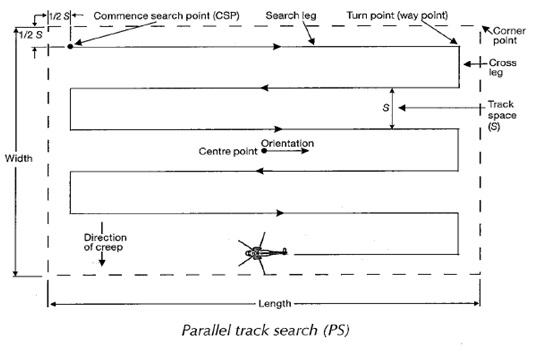
\includegraphics[width=\linewidth]{parallelSweepSearch.jpg}
	\label{fig:parallelSweep}	
	\end{figure}
	\footnotetext{image from: \url{http://marinegyaan.com} (May 2018)}
	
	The third algorithm developed in~\cite{Lin2009} is a discrete Genetic Algorithm-like EA.
	It is discussed how designing such an algorithm is challenging due to the nature of the problem meaning that the fitness of any given sequence of moves is entirely dependent on all of the previous moves leading to that sequence, and so an earlier sequence of moves drastically affects the fitness of any later sequence. 
	In other words, unlike the path planning problems addressed in~\cite{Yang2015} for planning a route between two points, this problem is not separable on waypoints. 
	With this in mind, they design a custom crossover and mutation strategy that allows quality sections of route to be exploited while still remaining in the bounded search area and also allowing for adequate exploration.
	The research conducted has also been applied more recently to a real world application using a quad-copter~\cite{Agcayazi2016}.
	
	In~\cite{Lin2014}, a number of algorithms are also proposed in a similar discretised problem space, where Gaussian Mixture Modelling is used to determine a number of clusters or regions of interest in the search space.
	The planners developed then use this information to derive a top level plan between the clusters and then look-ahead hill climbing to plan a route within each cluster.
	
	While the approach of placing a single fixed sensor in a cell at a constant altitude and a given time step has been shown to be successful in a simple wilderness search and rescue mission with a single known target and highly manoeuvrable quad-copter, the discritised nature makes it very challenging to extend the work directly to more complex, real-world scenarios.
	
	For instance, a real world UAV S\&R mission could involve optimising for multiple--possibly gimballed and optically zoom-able--sensors and multiple types of target. Gimballed sensors would therefore potentially require a secondary planning algorithm. The aircraft chosen would also likely be a fixed wing UAV due to the much longer flight duration and therefore could have highly constrained flight dynamics. The target probability distributions (or POC) could evolve over time--especially in a maritime setting where search objects are subject to ocean drift.
	Any of these factors would add significant complexity to the solution either through constraints in the solution space, or simply through computational complexity.
	As discussed in~\cite{Clark2013}, this stacking of complexity suggests that any algorithmic approaches would be best designed or adapted into some hierarchical planning model.
	
	In this paper, the problem is re-cast as a real-valued optimisation, which focusses on the flight path of the aircraft alone, enabling the work be potentially to be adopted as part of such a hierarchy or to be more easily expanded to incorporate some more of these complexities.
	
	
	In section~\ref{section:problem}, the search and rescue planning problem is presented in a more continuous form where the probability distribution is approximated using a Monte Carlo sampling approach~\cite{hastings1970monte} and a candidate solution is formed from a sequence of consecutive heading alterations. This reduces the dimensionality of the problem and should also allow for more obvious adaptation to real-world applications and future work, while encoding some level of flight dynamic constraints into the problem space itself.
	
	In section~\ref{section:algorithm}, an algorithm is designed based on JADE~\cite{Zhang2009}, but introduces two novel alterations. The first, to decode the headings into 2-dimensional waypoints prior to the mutation and crossover steps; and the second, to introduce a route freezing mechanism to act in a similar way the the SEW approach (\cite{Yang2015}\&\cite{Yang2016}) and to focus later generations of search on exploring the more temporally distant waypoints.
	
	Section~\ref{section:method} describes the analysis carried out. A number of example search scenarios are defined and comparison algorithms are chosen, with results and analysis in section~\ref{section:results}.
	Finally, section~\ref{section:conclusion} contains a brief conclusion and outlines several areas for future work.
	
	\section{Problem Description}	
	\label{section:problem}
	
	Mission planning for search and rescue is based on a field of mathmatics called search theory, that was initially developed in the second world war for the US military by B.O.Koopman~\cite{doi:10.1287/opre.4.3.324},~\cite{doi:10.1287/opre.4.5.503}\&~\cite{doi:10.1287/opre.5.5.613} to search for German U-Boats and downed aircraft. 
	The theory is formed using the Bayesian probability mathematics of detecting a particular target object. 
	
	\subsection{Probability of Detection}

	The main premise is that a searcher carries out some $n$ number of independent glimpses where $g$ is the probability that the object is detected at any particular glimpse. 
	This mathematically, forms a Bernoulli trial in which failures multiply.
	\begin{equation}
	\label{equation:glimpseProbability}
	p_n=1-(1-g)^n
	\end{equation}
	Where $p_n$ is the probability of detection (POD) after $n$ glimpses. 
	
	Since searching is continuous, and since each glimpse is independent, with the instantaneous probability of detection denoted as $\gamma$, it then follows that at time $t$:
	\begin{equation}
	\label{equation:continuousGlimpseProbability}
	P_d(t)=1-e^{-\gamma t}
	\end{equation}
	Where $P_d$ denotes the function describing the probability of detection after time $t$.
	
	Now, given that the searcher and the object would normally be in motion over time, the instantaneous probability of detecting the object $\gamma$ also changes in relation to time $t$.
	This, mathematically is an integration of a function $\gamma(t)$, which inserted into~(\ref{equation:continuousGlimpseProbability}), becomes:
	\begin{equation}
	\label{equation:integratedGlimpseProbability}
	P_d(t)=1-e^{-\int_{0}^{t} \gamma(t) dt}
	\end{equation}
	
	The glimpse probability $\gamma$ depends on many environmental factors such as the meteorological conditions, characteristics and visibility of the target, the searcher's facilities/sensors and altitude of the searcher.
	However, Koopman realised that many of these factors would be constant for a given search and could be measurable using further studies or analysis and inserted into data tables to cross reference for a given search.
	With this as an assumption, the only factors that would then vary throughout the search are the altitude $h$ and horizontal distance $r$ of the searcher to the target.
	
	Koopman used this to derive what is known as the inverse cube law of visual detection~\cite{doi:10.1287/opre.4.5.503}, which assumes that the rate of detection is proportional to the altitude $h$ and the inverse of the lateral range $s$ cubed.
	\begin{equation}
	\label{equation:lateralInverseSquareLaw}
	\gamma = \frac{kh}{s^3}
	\end{equation}
	Where $k$ is the constant describing all of the other measured factors of glimpse detection mentioned including the size of the target, visibility and meteorological conditions. 
	
	Given that the lateral distance $s$ can be derived from the altitude $h$ and horizontal distance $r$, it can also be calculated as:
	 \begin{equation}
	\label{equation:horizontalInverseSquareLaw}
	\gamma = \frac{kh}{(r^2+h^2)^{3/2}}
	\end{equation}
	
	This froms the basis of the probability of detection (POD) or $P_d$ devised by Koopman, and although there are other, more accurate models to calculate the POD~\cite{Washburn1993}, it should be an adequate estimation for the purposes of this work.
	This is especially true, since the aim of the algorithms developed in this paper are to optimise only the flight path, assuming that the plan for gimballed on-board sensors could be optimised by separate algorithm requiring more accurate approximations for the POD, for instance by projecting pixels onto the search area to calculate relative sizes of objects in the field of view.
	
	\subsection{Probability of Containment}	
	
	The POD alone assumes that the target is is covered by the area searched.
	In other words, POD can be probabilistically described as:
	$$
	P_d=p(detection | containment)
	$$ 
	The probability of containment (POC), denoted $p(containment)$ or $P_c$, is the second aspect of search theory and describes the probability of covering the location of the target in the search plan.
	
	The probability of success (POS), denoted $P_s$, of finding the object can therefore be described as the probabilistic conjunction of the POD and POC.
	$$
	P_s=p(detection \land containment)
	$$
	Which, becomes:
	$$
	P_s=p(containment) \times p(detection|containment)
	$$
	Or more succinctly for our purposes, written as:
	\begin{equation}
	\label{equation:probabilityOfSuccess}
	P_s=P_c \times P_d
	\end{equation}
	
	The POC is effectively an estimation of the 2-dimensional probability distribution of the target location covered by the search.
	Given the limited computational power available at the time of the second world war, this was roughly calculated, usually as a 2-dimension Gaussian distribution around a last known location or last known route.
	Some level of ocean drift estimation would then also be included with the standard deviation increasing over time.
	The overall search area would be divided into a uniformly discretised grid and the probability of containment value calculated for each cell in the grid.
	
	By defining a function $\phi(x,y)$, which maps 2-dimensional grid coordinates $x\in X$ and $y\in Y$ to the probability contained within a particular grid cell, the following can be derived:
	
	\begin{equation}
	\label{equation:gridProbability}
	\sum_{x,y\in X\times Y}\phi(x,y)=1
	\end{equation}
	
	Koopman uses the mathematics from the POD to define optimal sweep widths for conducting a parallel sweep search (see figure~\ref{fig:parallelSweep}) over a rectangular area that guarantees an area is covered uniformly and optimally by a human-controlled search craft. 
	This is achieved through integration of lateral range curves~\cite{doi:10.1287/opre.5.5.613}.
	If the grid cells covered by the uniform search by a particular search craft are represented as:
	$$
	C \subseteq X \times Y
	$$
	Where $X\in \{1,...,n\}$ and $Y\in \{1,...,m\}$.
	
	Then the probability of containment $P_c$ from searching the grid cells in $C$ can be calculated as:
	\begin{equation}
	\label{equation:gridPOC}
	P_c=\frac{\sum_{x,y\in C}\phi(x,y)}{\sum_{x,y\in X\times Y}\phi(x,y)}
	\end{equation}
	Or, due to the result in (\ref{equation:gridProbability}), more simply:
	\begin{equation}
	\label{equation:gridPOC}
	P_c=\sum_{x,y\in C}\phi(x,y)
	\end{equation}
	
	The $P_s$ of finding the target object after the search $C$ has been conducted can be calculated by using the appropriate value of $k$ from (\ref{equation:lateralInverseSquareLaw}) to estimate $P_d$, and then using (\ref{equation:probabilityOfSuccess}), to estimate the overall probability of success for the proposed search plan.
	Therefore, optimising the search plan involved defining optimal rectangular search areas assigned to the available search craft.
	
	This formed the main process of search and rescue mission planning until the early 1970s, when the US Coast Guard began developing the Computer Assisted Search Planning System (CASP)~\cite{Richardson1980}.
	The aim of CASP was effectively to provide a higher fidelity POC model and provide supporting functions to aid search asset mission planning. 
	Rather than using a discretised grid to represent the POC, the system uses a Monte Carlo sampling approach. 
	
	With this approach, the probability of containment distribution can be represented by randomly sampling $n$ particles $\rho_i=(x_i,y_i,\phi_i)$ from the configured initial probability distribution represented by a function, say $initialRand_c$, where $\phi_i$ is the probabilistic weighting of each particle, initialised as $\phi_i=1$, and $(x_i,y_i)=initialRand_c(),\forall i\in n$.
	The overall probability of containment can then be approximated as:
	
	\begin{equation}
	\label{equation:monteCarloPOC}
	\frac{\sum_{i=1}^{n}{\phi_i}}{n}=1
	\end{equation}	  
	
	Drift characteristics are used based on the search target object so that the particle locations can be updated over time according to environmental factors using an ocean drift model, such as developed in~\cite{Allen2006}.
	For a search at time $t$ covering an area $C_t \in X \times Y$, where $X \in \mathbb{R}$ and $Y \in \mathbb{R}$ representing real valued coordinates, the probability of detection for the area covered at time $t$ can be denoted $P_d(C_t)$. Since probability of failures multiply as in (\ref{equation:glimpseProbability}), the probability weighting of each particle $\phi_i \forall i\in n$ can be recursively updated for every new area searched.
	$$
	\phi_i^t=
	\begin{cases}
	\phi_i^{t-1}\cdot (1-P_d(C_t)), & \text{if } (x_i,y_i) \in C_t\\
	\phi_i^{t-1}, & \text{otherwise}
	\end{cases}
	$$
	Finally, the probability of success after search $C_t$, denoted $P_s(C_t)$ is then calculated as:
	
	\begin{equation}
	\label{equation:monteCarloPOS}
	P_s(C_t)=1-\frac{\sum_{i=1}^{n}{\phi_i^t}}{n}
	\end{equation}
	
	The planning aspect for CASP therefore still involved defining a number of parallel sweep searches to be conducted at particular times with the dimensions and locations of the rectangular areas optimised based on the POD characteristics and range of the available search craft.
	Optimising the search plan was then a question of optimising $P_s$ after all searches had been conducted.
	More recently developed S\&R planning systems (\cite{Liao2010},~\cite{ODonnell2006},~\cite{BREIVIK200899}\&~\cite{ABIZEID2005630}), although improving upon many of the underlying algorithms and planning functions as well as utilising dramatically improved computational power and environmental drift models, are based upon the same principle of optimising the assignment, locations and size of rectangular search areas for each available search craft.
	
	The reasons for this approach to S\&R planning are mostly due to the fact that conventional S\&R missions are conducted by manned craft.
	For such assets to search effectively, the optimal strategy is to use a predefined and easy to follow search pattern, which distributes search effort uniformly and, which can be communicated effectively using as few instructions as possible. 
	While the work in~\cite{Lin2009} and~\cite{Lin2014} attempts to produce more flexible and optimal search patterns for an autonomous craft, the use of a discretised search space presents a number of limitations as discussed in section~\ref{section:intro}.
	
	\subsection{Real Valued Fitness Function for a UAV Search Plan}
	
	The work in this paper, uses some of the mathematics from search theory to derive a more continuous fitness function for a route consisting of a number of waypoints in 2-dimensional space connected by straight line segments.
	It is observed that by using a Monte Carlo sampling approach to approximate the location probability distribution of the search object, it follows that each sampled particle represents an equal likelihood for the location of the target. 
	It is then possible to use the probability of detection calculation in (\ref{equation:integratedGlimpseProbability}) and the inverse cubed law of visual detection in (\ref{equation:horizontalInverseSquareLaw}) to directly calculate $P_s$ for a given search route using the arithmetic mean of the probabilities of detecting each individual particle.
	
	Say, for a given stationary particle $\rho_i$ at location $(x_{i},y_{i})$, and a route consisting of a single search leg at a constant altitude $h$ from waypoint $w_j$ at time $t=t_j$ and location $(x_{j},y_{j})$ to waypoint $w_{j+1}$ at time $t=t_{j+1}$ and location $(x_{j+1},y_{j+1})$, the instantaneous horizontal distance $r$ from the particle to the UAV at time $t$ (where $t_j\leq t \leq t_{j+1}$) can be calculated:

\begin{equation}
	\label{equation:particleWpDistance}
\begin{split}
r = (((x_{w^j}-x_{p^i})+(x_{w^{j+1}}-x_{w^j}) t)^2\\
 + ((y_{w^j}-y_{p^i})+(y_{w^{j+1}}-y_{w^j}) t)^2)^{1/2}
\end{split}
\end{equation}
	
	By incorporating this into equation (\ref{equation:horizontalInverseSquareLaw}) to denote the instantaneous probability of detection $\gamma(t)$ and then integrating this through $dt$ between $t=t_j$ and $t=t_{j+1}$ (see appendix~\ref{appendix:integratingInverseCubedLaw}), it is possible to calculate $P^i_d(t)$, the probability of detecting particle $\rho_i$ for any given segment of the route between $t_j$ and $t_{j+1}$ using equation (\ref{equation:integratedGlimpseProbability}).

	For multiple legs of a route with $m$ waypoints, each at time $t_j,\forall j \in m$, the probability of not detecting particle $\rho_i$, becomes:
		
		\begin{equation}
		\overline{P}_d^i(t_m)=e^{-\sum_{j=0}^{m-1}{\int_{t_j}^{t_{j+1}} \gamma(t) dt}}
		\end{equation}
	Further, because each sampled particle represents an equal portion of the overall probability distribution, the total probability of successfully finding the target $P_s$ after a proposed route, can be approximated as:
	
	\begin{equation}
	\label{equation:continuousWP-POS}
	P_s(t_m)=1-\frac{\sum_{i=1}^{n}{\overline{P}_d^i(t_m)}}{n}
	\end{equation}
	However, since algorithmic optimisation usually consists of minimising some function, the fitness function used in this work is the probabilistic inverse of the $P_s$, or rather the probability of not detecting the object after the route has been flown.
	
	\begin{equation}
	\label{equation:continuousWP-POSfitness}
	\overline{P}_s(t_m)=\frac{\sum_{i=1}^{n}{\overline{P}_d^i(t_m)}}{n}
	\end{equation}
	
	It is worth mentioning here that by using this approach to define a fitness function, it would be possible to extend (\ref{equation:particleWpDistance}) and the equations in appendix~\ref{appendix:integratingInverseCubedLaw} relatively trivially to account for routes with changing altitude and also problems with drifting particles--assuming that the particles drift linearly and at a constant rate between each time step $t_j$ and $t_{j+1}$. 
	However, for the purposes of simplicity, both of these will be assumed constant in this paper.
	Also, even though the proposed fitness function is computationally expensive, the number of computations can be directly adjusted by altering the number of particles $n$ to use a more or less approximate representation of the probability distribution.
	
	\subsection{Encoding Waypoints as Headings}
	
	Although the fitness function is designed to be calculated from times and positions of waypoints, this does not seem the best encoding of a route for the purposes of this optimisation problem.
	This is partly because encoding a solution as such produces a $3m$-dimensional problem where each waypoint $w_j$ requires 3 variables $(x_j,y_j,t_j)$, which results in much high dimensionality than is necessary.
	Further, encoding solutions in this manor means that the bounded search domain for each waypoint variable is large since $x_j$ and $y_j$ must be selected from some bounded search area $C\in X\times Y$.
	This encoding would also require that further constraints on the solutions be defined to ensure that $t_{j-1}\leq t_j \leq t_{j+1}$ and that $t_m \leq T$ where $T$ is the maximum flight time of the UAV search.
	If restrictions on flight dynamics are also included, as would be necessary in a real-world scenario, then more constraints on the solutions must be defined such as a maximum or minimum speed and turning angles between waypoints.
	These factors quickly transform the problem into what is effectively a multi-objective optimisation~\cite{Yang2015} with binary fitness functions to discard or constrain certain candidate solutions, adding complexity and hindering the performance of any selected optimisation algorithm.
	
	Instead, it is assumed that the UAV is flying at a constant speed between $m$ equally separated waypoints.
	When each waypoint is reached, the UAV makes a course change to fly towards the next waypoint.
	With this as an assumption, each waypoint can be represented by a single value--the heading alteration in radians $\theta$--and the candidate route as a sequence of such heading alterations $\theta_j, \forall j \in m$.
	Further, the flight dynamic constraints regarding maximum turning angle $\theta^{max}$ can be directly encoded as the bounds for each problem variable, serving to dramatically reduce the size of the search area to $[-\theta^{max},\theta^{max}]$ for all variables.
	
	The approach used for encoding the waypoints means that all candidate solutions must produce smooth and feasible flight trajectories within the maximum target flight range while also dramatically reducing the size of the search domain without introducing any additional problem constraints.
	In a way, this is a similar--but more extreme--concept to the rotated coordinate representation proposed in~\cite{Yang2014}.
		
	\section{Proposed Algorithm}
	\label{section:algorithm}
	
	Given the successes in~\cite{Yang2015}, the chosen algorithm to be applied to the problem is based on JADE~\cite{Zhang2009}.
	JADE is an adaptive version of Differential Evolution (DE) algorithm, which is itself a simple and elegant but extremely effective evolutionary algorithm that has been successfully applied to many real-world optimisation applications (\cite{storn1997differential},~\cite{mezura2006comparative},~\cite{Das2011}).
	DE has a 1-to-1 mutation and crossover strategy where the mutation is generated from a number of randomly selected individuals in the population. 
	The original implementation of DE~\cite{storn1997differential}, uses:
	\begin{equation}
	\label{equation:originalDEMutation}
	v_i=x_{r_1}+F(x_{r_2}-x_{r_3})
	\end{equation}
	Where $v_i$ is the mutated solution vector, $x_{r_1} \neq x_{r_2} \neq x_{r_3}$ are three randomly chosen individual solutions from the population $P$ and $F$ is the pre-defined mutation factor parameter (usually chosen between $0.5$ and $1$).
	The crossover strategy can either be binomial, where each variable has an equal probability to be selected for crossover with the mutated solution; or exponential, where a burst of variables are crossed over with exponentially decreasing probability.
	The crossover is controlled by parameter $CR$, usually in the range $[0.8,1]$ (\cite{Liu2005}).
	
	\subsection{JADE}
	
	As mentioned in~\cite{Zhang2009}, the performance of DE is often dependent on the choice of the mutation parameter $F$ and the crossover probability $CR$ and algorithms which adapt these parameters dynamically to the problem can achieve far greater convergence performance.
	While there are a number of adaptive implementations of DE, JADE is based on an implementation of a greedy variant of DE (DE/current-to-best/1/bin), for the reason of favouring fast convergence over reliability for use in an adaptive DE.
	
	\begin{algorithm}[h]
  \caption{JADE with Archive}\label{algorithm:JADEwArchive}
  \begin{algorithmic}[1]
    \Procedure{JADE}{}
    \State Set $\mu_{CR}=0.5$; $\mu_{F}=0.5$; $A=\emptyset$
    \State Set random initial population: $ \{x_{i,0}|1,2,..NP \}$
    \For{$g=1$ to $G$}
    \State $S_F=\emptyset$; $S_{CR}=\emptyset$
    \For{$i=1$ to $NP$}
    \State Set $CR_i=randn(\mu_{CR},0.1)$
    \State Set $F_i=randn(\mu_{F},0.1)$
    \State Random $x_{best}^p$ from top $100p\%$ in $P_g$
    \State Random $x_{r1,g} \neq x_{i,g}$ from $P_g$
    \State Random $\widetilde{x}_{r2,g} \neq x_{r1,g} \neq x_{i,g}$ from $P_g \cup A$
	\State $v_{i,g}=x_{i,g} + F_i \cdot (x^p_{best}-x_{i,g})+ F_i \cdot (x_{r1}-\widetilde{x}_{r2})$
	\State Random $j_{rand}=randint(1,D)$
	\For{$j=1$ to $D$}
	\If{$j=j_{rand}$ OR $rand(0,1)<CR_i$}
	\State $u_{j,i,g} = v_{j,i,g}$
	\Else
	\State $u_{j,i,g} = x_{j,i,g}$
	\EndIf
	\EndFor
	\If{$f(x_{i,g}) \leq f(u_{i,g})$}
	\State $x_{i,g+1}=x_{i,g}$
	\Else
	\State $x_{i,g+1}=u_{i,g}$; $x_{i,g} \rightarrow A$
	\State $CR_i \rightarrow S_{CR}$; $F_i \rightarrow S_F$
	\EndIf
    \EndFor
    \State Randomly remove from $A$ until $|A| \leq a$
    \State $\mu_{CR}=(1-c) \cdot \mu_{CR} + c \cdot mean_A(S_{CR})$
    \State $\mu_F=(1-c) \cdot \mu_F + c \cdot mean_L(S_F)$
    \EndFor
    \EndProcedure
  \end{algorithmic}
\end{algorithm}

	JADE introduces a new mutation strategy (DE/current-to-pbest), where each mutated vector uses a candidate chosen $x^p_{best}$ from the top $100p\%$ of the population, and $p\in (0,1]$ is a constant, pre-defined parameter.
	This serves to make the mutation strategy more diverse (less greedy) than DE/current-to-best.
	The new mutation strategy is defined as:
	\begin{equation}
	\label{equation:JADEMutation}
	v_i=x_i + F_i \cdot (x^p_{best}-x_i)+ F_i \cdot (x_{r_1}-x_{r_2})
	\end{equation}
	Where $x_i$ is the current individual in the the population. The mutation factor $F_i$ is randomly sampled from a Cauchy distribution $randc(\mu_F,0.1)$ for each $i$th individual in a generation.
	The crossover probability $CR_i=randn(\mu_{CR},0.1)$ is also sampled from a normal distribution for each $i$th individual from the population.
	The binomial crossover strategy is then applied.
	
	JADE can also use an archive $A$ of discarded individuals from previous generations.
	If this is in use, then the mutation vector becomes:
	\begin{equation}
	\label{equation:JADEMutationArchive}
	v_i=x_i + F_i \cdot (x^p_{best}-x_i)+ F_i \cdot (x_{r_1}-\widetilde{x}_{r_2})
	\end{equation}
	Where $\widetilde{x}_{r_2}$ is randomly selected from $P \cup A$.
	Individuals are added to the archive if they are out competed by their mutated sibling at selection.
	Random individuals are then removed from the archive at the end of each generation so that $|A| \leq a$ (where $a$ is a predefined parameter denoting the maximum size of the archive).
	
	As well as this, the successful $CR_i$ and $F_i$ are added to a cache of successful crossover probabilities $S_{CR}$ and a cache of successful mutation factors $S_F$ for that particular generation. The values of $\mu_{CR}$ and $\mu_F$ (both initialised as $0.5$) can then be updated at the end of each generation according to the following:
	\begin{equation}
	\label{equation:JADEAdaptionCR}
	\mu_{CR}=(1-c) \cdot \mu_{CR} + c \cdot mean_A(S_{CR})
	\end{equation}
	\begin{equation}
	\label{equation:JADEAdaptionF}
	\mu_F=(1-c) \cdot \mu_F + c \cdot mean_L(S_F)
	\end{equation}
	Where $c\in (0,1)$ is the constant adaptation parameter, $mean_A$ is the arithmetic mean and $mean_L$ is the Lehmer mean, calculated as:
	\begin{equation}
	\label{equation:LehmerMean}
	mean_L(S_F)=\frac{\sum_{F\in S_F}{F^2}}{\sum_{F\in S_F}{F}}
	\end{equation}
	
	The pseudo code for JADE, taken from~\cite{Zhang2009}, can be seen in algorithm~\ref{algorithm:JADEwArchive}.
	
	\subsection{Decoding Waypoints}
	
	Since an individual $x_{i,g}$ from the population $P_g$ is encoded as a sequence of headings from one waypoint location to the next, the information about the quality of each heading $x_{i,j,g}$ is entirely dependant on all previous headings from $x_{i,0,g}$ to $x_{i,j,g}$.
	This presents an issue at the mutation and crossover steps whereby altering $x_{i,j,g}$ using the information from some another individual, say $x_{\sigma,j,g}$ with $\sigma \in NP$, the information contained in $x_{\sigma,j,g}$ is meaningless in the context of $x_{i,j,g}$ because the previous headings leading up to $x_{\sigma,j,g}$ could be completely different to the previous headings leading up to $x_{i,j,g}$.
	
	To address this issue, the first alteration to JADE is proposed.
	Rather than executing the mutation and crossover steps directly on each $x_{i,j,g}$, the heading values of the individual can be transformed back into a vector of waypoints $w^x_{i,j,g},w^y_{i,j,g}$ using a function such as described in algorithm~\ref{algorithm:DecodingWaypoints}.
	
	\begin{algorithm}[h]
  \caption{Decoding Waypoints}\label{algorithm:DecodingWaypoints}
  \begin{algorithmic}[1]
    \Procedure{DecodeWaypoints}{x}
    \State Set $s_x,s_y$ as predefined start location
    \State Set $d$ as predefined waypoint distance
    \State Set $w^x_{0}=s_x$; $w^y_{0}=s_y$
    \State Set heading $h=0$
    \For{$j=1$ to $D$}
    \State $h=h+x_j$
    \State $w^x_j=w^x_{j-1}+\sin{x_j} \cdot d$
    \State $w^y_j=w^y_{j-1}+\cos{x_j} \cdot d$
    \EndFor
    \State Return {$w$}
    \EndProcedure
  \end{algorithmic}
\end{algorithm}
	
	Once the mutated vector $v_{i,g}$ has been generated--now consisting of a sequence of waypoints--the crossover step encodes and re-saturates the chosen waypoints back into a vector of bounded heading alterations.
	This means that if a particular waypoint is chosen for crossover, then the new heading derived from that crossover should  always aim the trajectory of the flight path in the direction of the chosen waypoint. In a sense this makes use of the fully derived or fully qualified information of that crossover and mutation choice.
	The pseudo code for this alteration to JADE can be seen in algorithm~\ref{algorithm:JADEwDecodingWaypoints}.
	For the sake of reducing computational load, the waypoint vectors in the actual implementation can be stored once calculated for the next generation.
	 
	 \begin{algorithm}[h]
  \caption{JADE with Decoded Mutation Step}\label{algorithm:JADEwDecodingWaypoints}
  \begin{algorithmic}[1]
    \Procedure{JADE-DecodedWaypoints}{}
    \State Set $\mu_{CR}=0.5$; $\mu_{F}=0.5$; $A=\emptyset$
    \State Set random initial population: $ \{x_{i,0}|1,2,..NP \}$
    \State Set $\theta^{max}$ as predefined maximum turn angle
    \For{$g=1$ to $G$}
    \State $S_F=\emptyset$; $S_{CR}=\emptyset$
    \For{$i=1$ to $NP$}
    \State Set $CR_i=randn(\mu_{CR},0.1)$
    \State Set $F_i=randn(\mu_{F},0.1)$
    \State Random $x_{best}^p$ from top $100p\%$ in $P_g$
    \State Random $x_{r1,g} \neq x_{i,g}$ from $P_g$
    \State Random $\widetilde{x}_{r2,g} \neq x_{r1,g} \neq x_{i,g}$ from $P_g \cup A$
    \State Set $w_{i,g}=DecodeWaypoints(x_{i,g})$
    \State Set $w_{best}^p=DecodeWaypoints(x_{best}^p)$
    \State Set $w_{r1,g}=DecodeWaypoints(x_{r1,g})$
    \State Set $\widetilde{w}_{r2,g}=DecodeWaypoints(\widetilde{x}_{r2,g})$
	\State $v_{i,g}=w_{i,g} + F_i \cdot (w^p_{best}-w_{i,g})+ F_i \cdot (w_{r1}-\widetilde{w}_{r2})$
	\State Set $q_{0,i,g}=w_{0,i,g}$; $\alpha=0$
	\State Random $j_{rand}=randint(1,D)$
	\For{$j=1$ to $D$}
	\If{$j=j_{rand}$ OR $rand(0,1)<CR_i$}
	\State $q_{j,i,g} = v_{j,i,g}$
	\State $dx= v^x_{j,i,g}-q^x_{(j-1),i,g}$
	\State $dy= v^y_{j,i,g}-q^y_{(j-1),i,g}$
	\Else
	\State $q_{j,i,g} = x_{j,i,g}$
	\State $dx= x^x_{j,i,g}-q^x_{(j-1),i,g}$
	\State $dy= x^y_{j,i,g}-q^y_{(j-1),i,g}$
	\EndIf
	\State $\theta_j = atan(dx,dy)$
	\State $u_{j,i,g}=min(max(\theta_j-\alpha,-\theta^{max}),\theta^{max})$
	\State $\alpha = \alpha + u_{j,i,g}$\Comment{Update previous heading}
	\EndFor
	\If{$f(x_{i,g}) \leq f(u_{i,g})$}
	\State $x_{i,g+1}=x_{i,g}$
	\Else
	\State $x_{i,g+1}=u_{i,g}$; $x_{i,g} \rightarrow A$
	\State $CR_i \rightarrow S_{CR}$; $F_i \rightarrow S_F$
	\EndIf
    \EndFor
    \State Randomly remove from $A$ until $|A| \leq a$
    \State $\mu_{CR}=(1-c) \cdot \mu_{CR} + c \cdot mean_A(S_{CR})$
    \State $\mu_F=(1-c) \cdot \mu_F + c \cdot mean_L(S_F)$
    \EndFor
    \EndProcedure
  \end{algorithmic}
\end{algorithm}
	
	\subsection{Temporal Route Freezing}
	
	Another issue observed is that executing mutation and crossover on an entire individual might prevent later generations of the population from exploiting more temporally distant waypoints because the locations of these are so greatly affected by the sequence of waypoints leading up to them.
	If all generations of the optimisation are able to alter earlier waypoints as much as later waypoints, with a diverse enough population, this could mean that the optimisation stagnates as individuals from different modes of the search space are selected at the mutation step.
	
	In order to reduce this effect and increase the speed of convergence, another alteration is made to the algorithm by using an extra saturation step with the aim of limiting change in heading variable $u_{j,i,g}$ from the previous individual $x_{j,i,g}$.
	This is achieved by calculating scaling factor $\psi_{j,g} \in (0,2)$ for each particular course adjustment $j\in D$ of a particular generation $g \in G$. This is then multiplied by the problem bounds $-\theta^{max}$ and $\theta^{max}$ to determine how much saturation to apply to $u_{j,i,g}$ from the previous heading $x_{j,i,g}$. The calculation for $\psi_{j,g}$ is shown below in (\ref{equation:exponentialFreezing}), and the updated pseudo code with the saturation step added in algorithm~\ref{algorithm:JADEwFreezing}. 
	
	\begin{equation}
	\label{equation:exponentialFreezing}
	\psi_{j,g} = 2e^{-((1-\frac{j}{D}) \cdot \frac{g}{G} \cdot \beta)}
	\end{equation}		
	Where $\beta$ is a predefined freezing parameter that determines how much "freezing" is applied, with a higher value causing more freezing.
	
	
	\begin{algorithm}[h]
  \caption{JADE with Temporal Route Freezing}\label{algorithm:JADEwFreezing}
  \begin{algorithmic}[1]
    \Procedure{JADE-RouteFreezing}{}
    \State Set $\mu_{CR}=0.5$; $\mu_{F}=0.5$; $A=\emptyset$
    \State Set random initial population: $ \{x_{i,0}|1,2,..NP \}$
    \State Set $\theta^{max}$ as predefined maximum turn angle
    \For{$g=1$ to $G$}
    \State $S_F=\emptyset$; $S_{CR}=\emptyset$
    \For{$i=1$ to $NP$}
    \State Set $CR_i=randn(\mu_{CR},0.1)$
    \State Set $F_i=randn(\mu_{F},0.1)$
    \State Random $x_{best}^p$ from top $100p\%$ in $P_g$
    \State Random $x_{r1,g} \neq x_{i,g}$ from $P_g$
    \State Random $\widetilde{x}_{r2,g} \neq x_{r1,g} \neq x_{i,g}$ from $P_g \cup A$
    \State Set $w_{i,g}=DecodeWaypoints(x_{i,g})$
    \State Set $w_{best}^p=DecodeWaypoints(x_{best}^p)$
    \State Set $w_{r1,g}=DecodeWaypoints(x_{r1,g})$
    \State Set $\widetilde{w}_{r2,g}=DecodeWaypoints(\widetilde{x}_{r2,g})$
	\State $v_{i,g}=w_{i,g} + F_i \cdot (w^p_{best}-w_{i,g})+ F_i \cdot (w_{r1}-\widetilde{w}_{r2})$
	\State Set $q_{0,i,g}=w_{1,g}$; $\alpha=0$
	\State Random $j_{rand}=randint(1,D)$
	\For{$j=1$ to $D$}
	\If{$j=j_{rand}$ OR $rand(0,1)<CR_i$}
	\State $q_{j,i,g} = v_{j,i,g}$
	\State $dx= v^x_{j,i,g}-q^x_{(j-1),i,g}$
	\State $dy= v^y_{j,i,g}-q^y_{(j-1),i,g}$
	\Else
	\State $q_{j,i,g} = x_{j,i,g}$
	\State $dx= x^x_{j,i,g}-q^x_{(j-1),i,g}$
	\State $dy= x^y_{j,i,g}-q^y_{(j-1),i,g}$
	\EndIf
	\State $\psi_{j,g} = 2e^{-((1-\frac{j}{D}) \cdot \frac{g}{G} \cdot \beta)} \cdot \theta^{max}$
	\State $\theta_j = atan(dx,dy) - \alpha + x_{j,i,g}$
	\State $\widehat{\theta}_j = min(max(\theta_j,-\psi_{j,g}),\psi_{j,g})-x_{j,i,g}$
	\State $u_{j,i,g}=min(max(\widehat{\theta}_j,-\theta^{max}),\theta^{max})$
	\State $\alpha = \alpha + u_{j,i,g}$\Comment{Update previous heading}
	\EndFor
	\If{$f(x_{i,g}) \leq f(u_{i,g})$}
	\State $x_{i,g+1}=x_{i,g}$
	\Else
	\State $x_{i,g+1}=u_{i,g}$; $x_{i,g} \rightarrow A$
	\State $CR_i \rightarrow S_{CR}$; $F_i \rightarrow S_F$
	\EndIf
    \EndFor
    \State Randomly remove from $A$ until $|A| \leq a$
    \State $\mu_{CR}=(1-c) \cdot \mu_{CR} + c \cdot mean_A(S_{CR})$
    \State $\mu_F=(1-c) \cdot \mu_F + c \cdot mean_L(S_F)$
    \EndFor
    \EndProcedure
  \end{algorithmic}
\end{algorithm}
%	
%	
%	
%	Issue is that doing so, you don't encode location since this is determined by previous moves.
%	
%	Sets the best first move first, takes the longest on this. Chooses based on scores from whole route, even though only the first waypoint gets set.
%	
%	Goes from move to move and sets the previous set of points?
%	
%	....
%	
%	Parameter choice...
	
	\section{Simulation}
	\label{section:method}
	
	In order to verify the proposed approach to planning a UAV path for search missions and to assess the impact of the two alterations made to JADE for this problem domain, three different scenarios are devised with increasingly complex initial probability distributions.
	In each scenario, the proposed planner is compared against 4 other real-valued optimisation algorithms and the results are analysed using a number of performance metrics.
	The routes generated by the optimisers can also be visualised to inspect subjectively whether the approach is able to produce sensible routes for a UAV carrying out such a mission.
	
	\subsection{Description of Scenarios}
	For each scenario, particles are initially sampled from predefined probability distributions made up from a number of equally probable, 2-dimensional Gaussian functions defined within the general--although not restricted--search area of $X\times Y$ with $X\in[0,1000],Y\in[0,1000]$.
	The number of particles $n$ is chosen to be $n=1000$ for all scenarios, so for a scenario consisting of $2$ Gaussian distributions, $500$ particles would be sampled from each.
	
	The number of waypoints $D$ is chosen to be $D=50$ for the first scenario and $D=100$ for the second and third scenario with distance between waypoints $d=100$ and the start location of the search is $s_x=500,s_y=500$.
	Given that the problem bounds $\alpha^{max}=\frac{\pi}{3}$ is also set as the same for all waypoints within each scenario, the paths always start in roughly the same direction of $\pm \frac{\pi}{3}$ radians.
	The time between waypoints is arbitrarily chosen as $t_{j+1}-t_j=2.0$ for all scenarios, and similarly an altitude of $h=500$ and glimpse detection constant $k=5.0e2$ are used to calculate the probability of detecting any given particle over the course of a generated route.
	
	The first search scenario (as can be seen in figures~\ref{fig:scenario1Good} and~\ref{fig:scenario1Poor}) involves a single Gaussian distribution directly in front of the first waypoint with $X\sim \mathcal{N}(500,62.5)$ and $Y\sim \mathcal{N}(800,62.5)$.
	The aim of this scenario is to test the performance of the algorithms in a simplistic setting and act as a base comparison for the selected algorithms.
	
	 The second and more complex scenario (as can be seen in figures~\ref{fig:scenario2Good} and~\ref{fig:scenario2Poor}) consists of $5$ distributions with $200$ particles sampled from each.
	 The first Gaussian is situated in the middle of the search area effectively surrounding the start location of the UAV, it also has a relatively small standard deviation with:
	  $$X_1\sim\mathcal{N}(500,33.3); Y_1\sim \mathcal{N}(500,33.3)$$
	 Four more distributions surround the first symmetrically with: 
	 $$X_2\sim \mathcal{N}(250,62.5);Y_2\sim \mathcal{N}(250,62.5)$$
	 $$X_3\sim \mathcal{N}(250,33.3);Y_3\sim \mathcal{N}(750,33.3)$$
	 $$X_4\sim \mathcal{N}(750,33.3);Y_4\sim \mathcal{N}(250,33.3)$$
	 $$X_5\sim \mathcal{N}(750,62.5);Y_5\sim \mathcal{N}(750,62.5)$$
	 This serves to test the greediness of the algorithms since an optimal strategy would be to visit each distribution for an equal duration but the central distribution might attract the algorithm to produce a path that stays in the middle of the search area.
	 This is also more multi-modal as the planners could choose to visit any of the distributions in any order and still produce a similar POS.
	 
	 Due to the symmetrical nature of the second search scenario, sections of a successful route in one mode of the search space could be crossed over for use in a route in a different mode of the search space and still be beneficial.
	 Therefore the third scenario (as can be seen in figures~\ref{fig:scenario3Good} and~\ref{fig:scenario3Poor}) is more complex again and is made from $5$ distributions also all containing $200$ particles each, but are all situated at irregular locations in the search area with vastly different shapes and sizes. The Gaussian distributions for scenario three are defined as:
	 $$X_1\sim\mathcal{N}(200,50); Y_1\sim \mathcal{N}(300,33.3)$$
	 $$X_2\sim \mathcal{N}(900,50);Y_2\sim \mathcal{N}(900,62.5)$$
	 $$X_3\sim \mathcal{N}(700,25);Y_3\sim \mathcal{N}(400,25)$$
	 $$X_4\sim \mathcal{N}(300,50);Y_4\sim \mathcal{N}(800,33.3)$$
	 $$X_5\sim \mathcal{N}(1000,100);Y_5\sim \mathcal{N}(100,20)$$
	 The third scenario aims to test and compare the performance of the algorithms at being able to generation routes for more complex initial conditions when there is not a visibly clear strategy.
	
	\subsection{Compared Algorithms}
	Four algorithms were chosen to be compared against the proposed algorithm~\ref{algorithm:JADEwFreezing}.
	Two of these are discussed in the paper, which are the JADE-DecodedWaypoints in algorithm~\ref{algorithm:JADEwDecodingWaypoints} and also the original JADE with archive as can be seen in algorithm~\ref{algorithm:JADEwArchive}.
	All three JADE-like algorithms use the same parameters to ensure a fair comparison with an adaption rate $c=0.08$ and top $100p\%$, with $p=0.05$. These are chosen within the suggested bounds in~\cite{Zhang2009} and based on some initial analysis of effective values for this problem domain.
	The population size used is $NP=10D=500$ (based on the size of the routes in scenario one), as the proposed size for DE algorithms, suggested in~\cite{Liu2005}. The maximum archive size is chosen as $a=2000$, which is $4NP$.
	The additional freezing coefficient used in the proposed algorithm is $\beta = 2.0$.
	
	An implementation of the original DE~\cite{storn1997differential} (DE/rand/1/bin) was also used to compare against the other selected algorithms.
	This uses the mutation strategy in (\ref{equation:originalDEMutation}), with binomial crossover.
	The parameters for this algorithm were also chosen from the recommended ranges in~\cite{Liu2005} as $F=0.75$ and $CR=0.9$ with the population size the same as the JADE implementations ($NP=500$).
	
	The final algorithm implemented to compare against the proposed algorithms is Simulated Annealing (SA)~\cite{S.KirkpatrickC.D.GelattJr.1983} with exponential cooling.
	This is a stochastic, single solution optimisation algorithm, which attempts to mimic the practice used in metallurgy to strengthen the material through heating and rapid cooling.
	Each repetition of cooling allows the molecules in the metal to transition to a more stable--and therefore stronger--arrangement.
	The algorithm uses a temperature parameter, which decreases over time.
	This parameter represents the probability of the solution exploring a distant solution and therefore controls the exploration behaviour of the algorithm.
	As the temperature cools, the algorithm favours a more exploitative strategy.
	
	While this algorithm has seen more successful applications to discrete optimisation problems~\cite{Kirkpatrick1984}, it serves as a reasonable baseline to compare against for our purposes.
	The parameters used for this algorithm are initial temperature $T=1.0e9$, minimum temperature $T_0=0.0$, perturbation factor $p=0.4$ and exponential cooling rate $c=0.8$.
	
	\subsection{Implementation and Performance Measures}
	
	The algorithms were implemented in Java using a framework of libraries provided by De Montfort University for developing and analysing the performance of real-valued optimisation algorithms on various problems.
	The framework computes the results for each algorithm on each problem for a set number of repeated iterations, in this case chosen to be 15, and generates text files for each run containing the final output solution and the fitness of the best solution at predetermined set intervals (in this case chosen to be after each generation or every 500 iterations for SA).
	The computational budget is calculated using a budget scaling factor of $4000$. This is multiplied by the dimensions of the problem space to calculate the overall budget for each experiment. This works out as $2.0e6$ computations for the first scenario, which for the population based algorithms amounts to $400$ generations and $4.0e6$ for the second and third scenario, which amounts to $800$ generations.
	The mean and standard deviation is then calculated for the fitness of the final output solution generated after each run.
	A Wilcoxon signed-rank score is also produced to compare the results of the proposed algorithm against each of the comparison algorithms over all of the repeated runs.
	This provides a statistical analysis of whether the proposed algorithm reliably outperforms or dominates any other selected algorithm based on their mean ranks.
	
	Another metric used to compare the results of the experiment is to calculate the median fitness from all runs of the algorithms after every generation (or after every 500 iterations of SA).
	This can then be plotted on a graph to get a sense of how quickly each algorithm converges.
	
	An application was also designed using the JavaFX framework to visualise the output solutions produced in order to determine their subjective quality.
	The paths are displayed on a 2-dimensional grid, with the particles also depicted as red circles in order to visualise the POC distribution.
	
	\section{Results and Analysis}	
	\label{section:results}

The results of the Wilcoxon signed-rank test against the comparison algorithms for all three scenarios can be seen in table~\ref{table:wilcoxonRanks}.
Interestingly, the proposed algorithm performs better in all three scenarios than most of the other algorithms, including--for the two more complex scenarios--the version of JADE with only decoded waypoints. 
This might imply that the proposed route freezing mechanism has a positive effect on the ability to find quality routes.
However, JADE with no route freezing or decoded waypoints, still outperforms the proposed algorithm in all three scenarios.

These results suggest, therefore, that the first proposed alteration of decoding the solutions into waypoints before mutation, might actually act as a hindrance to the algorithm.
The second alteration of freezing the routes may be beneficial, although this alteration is combined with the first so more analysis here is required to confirm whether route freezing without decoding the waypoints would still be beneficial.

%
%
%
%Interesting observation of overfitting when low glimpse probability factor due to the inverse cube law.	
%	How many runs..?\\
%	
	
	\begin{table}[t]
\centering
\caption{Table of Wilcoxon Signed Rank Against Proposed Algorithm}
\label{table:wilcoxonRanks}
\begin{tabular}{c|cll|}
\cline{2-4}
\multicolumn{1}{l|}{}                       & \multicolumn{3}{l|}{\textbf{Scenario}} \\
\multicolumn{1}{l|}{\textbf{}}              & \multicolumn{1}{l}{1}    & 2    & 3    \\ \hline
\multicolumn{1}{|c|}{\textbf{SA}}                    & +               & +    & +    \\
\multicolumn{1}{|c|}{\textbf{DE/rand/1/bin}}         & +               & +    & +    \\
\multicolumn{1}{|c|}{\textbf{JADE}}                  & -               & -    & -    \\
\multicolumn{1}{|c|}{\textbf{JADE-DecodedWaypoints}} & =               & +    & +    \\ \hline
\end{tabular}
\end{table}
	
\begin{figure}[t]
	\caption{Error Bars Showing Means and Standard Deviations for Scenario 1}
	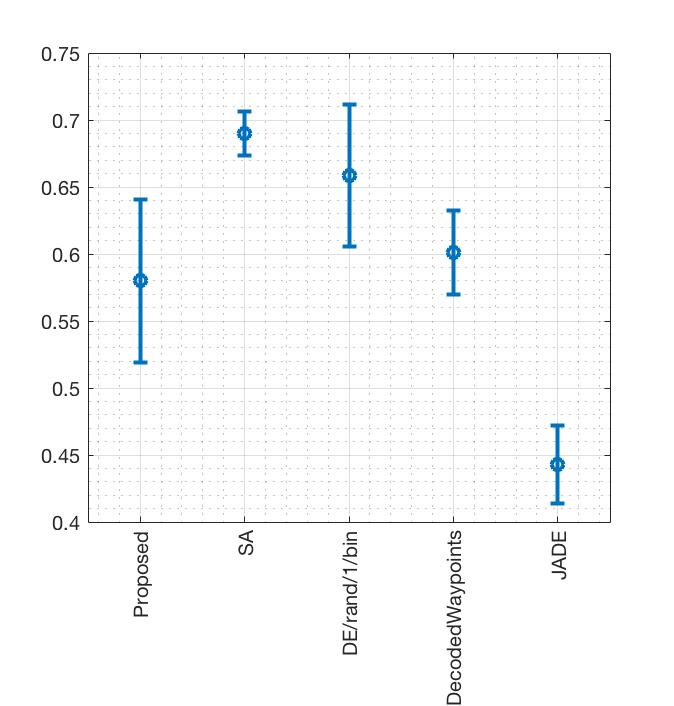
\includegraphics[width=0.8\linewidth]{scenario1Means.jpg}
	\centering
	\label{fig:scenario1Means}	
	\end{figure}
	
\begin{figure}[t]
	\caption{Error Bars Showing Means and Standard Deviations for Scenario 2}
	\centering
	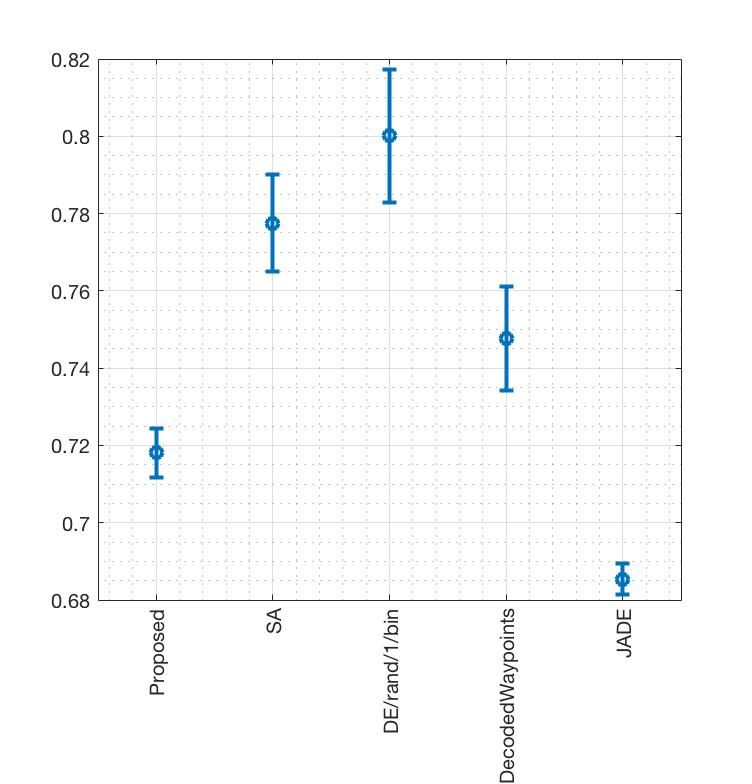
\includegraphics[width=0.8\linewidth]{scenario2Means.jpg}
	\label{fig:scenario2Means}	
	\end{figure}
	
	\begin{figure}[t]
	\caption{Error Bars Showing Means and Standard Deviations for Scenario 3}
	\centering
	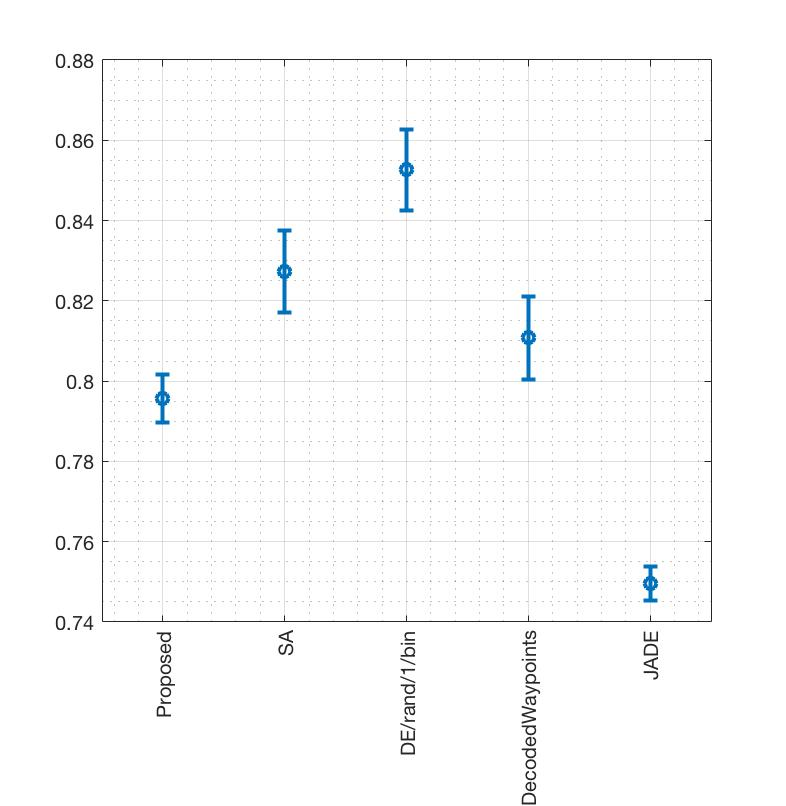
\includegraphics[width=0.8\linewidth]{scenario3Means.jpg}
	\label{fig:scenario3Means}	
	\end{figure}	
	
The box plots in figures~\ref{fig:scenario1Means},~\ref{fig:scenario2Means} and~\ref{fig:scenario3Means} show the mean fitness and standard deviation of the final routes for scenarios 1, 2 and 3 respectively over the 15 runs of the experiment.
These also seem to confirm that JADE significantly outperforms the proposed algorithm in all three scenarios, especially in the more complex scenarios.
The proposed algorithm has the second best average fitness in all three scenarios with the algorithm that only has decoded waypoints and no route freezing, close third.

In scenario 1, the proposed algorithm produces a large range in fitness of the routes produced and appears to not perform any better than the version with no route freezing, which is also confirmed by the Wilcoxon rank.

Interestingly, the box plots for the second two scenarios also appear very similar, which could be partly due to the fact that they have the same length of routes and number of generations.
This adds to the reliability of the results as it demonstrates some level repeatability.
It also suggests that there is no relative difference in performance between the algorithms finding routes in a symmetrical distribution such as scenario 2 compared to a non-symmetrical or more random distribution in scenario three.
Further it could imply that none of the algorithms are more prone to greediness in scenario 2 (with a central distribution) than the others--when compared relatively.

When optimisation algorithms perform poorly, it can normally be put down to one of two causes. The first of these is that the algorithm converges too early on a local optima and then lacks the diversity and exploration capacity to discover a better optima.
The second reason is that the algorithm stagnates, where there are essentially too many avenues of exploration preventing the algorithm from exploiting a solution in any one direction.

In the case of the proposed algorithm, it is somewhat difficult to discern which of these reasons contribute to the poor performance of the proposed algorithm.
It is generally considered that DE algorithms are very prone to stagnation due to mutated candidates being generated from a number of other candidates potentially "pulling" the solutions in all directions at every iteration.
However, given that the alteration to JADE is aimed at speeding up convergence by mutating based on the information in the 2-dimensional waypoints, this might suggest the contrary.

Another observation to note from the mean data plots is that SA appears to perform slightly better than DE, especially in the more complex scenarios.
It could be partly due to the lack of adequate parameter tuning for the DE algorithm.
However, another explanation for this could be stagnation, which, as mentioned, DE is quite prone. 
On the other hand SA is generally much more of a greedy algorithm.
It would seem that for this problem, it pays to be somewhat greedy, which would make sense because intuitively for these scenarios, there would be a great number of paths (or modes) that would lead to similar fitness. This is especially true in the more symmetrical scenarios.



\begin{figure}[H]
	\caption{Scenario 1 - Example of Poor Route ($\overline{P}_s(t_m)=0.681$)}
	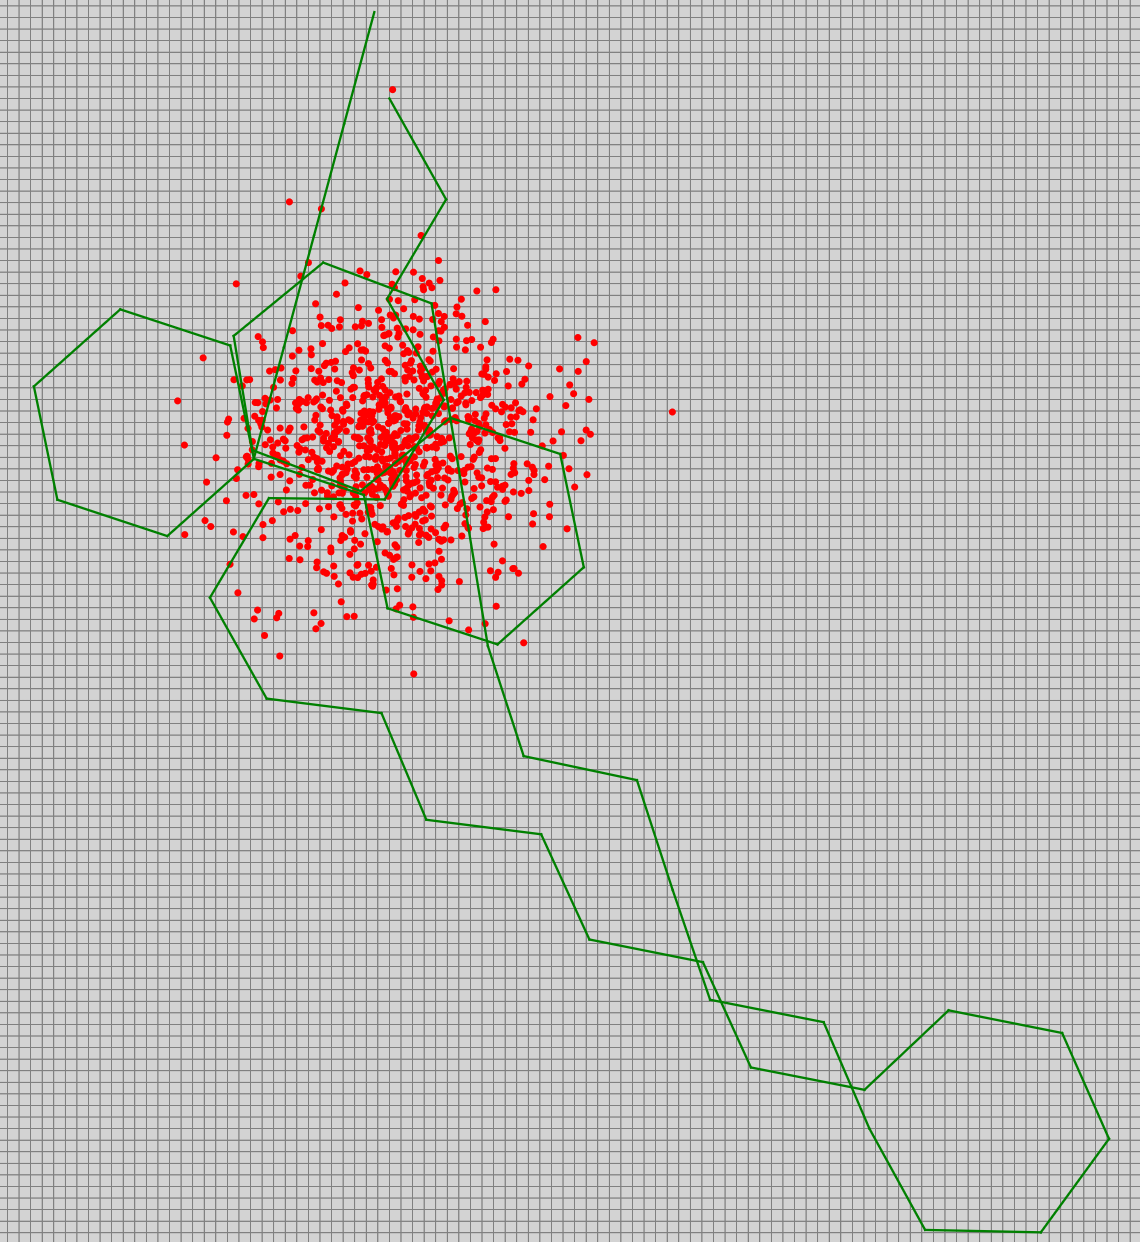
\includegraphics[width=0.7\linewidth]{poorRouteScenario1.png}
	\centering
	\label{fig:scenario1Poor}	
	\end{figure}

\begin{figure}[H]
	\caption{Scenario 1 - Example of Good Route ($\overline{P}_s(t_m)=0.509$)}
	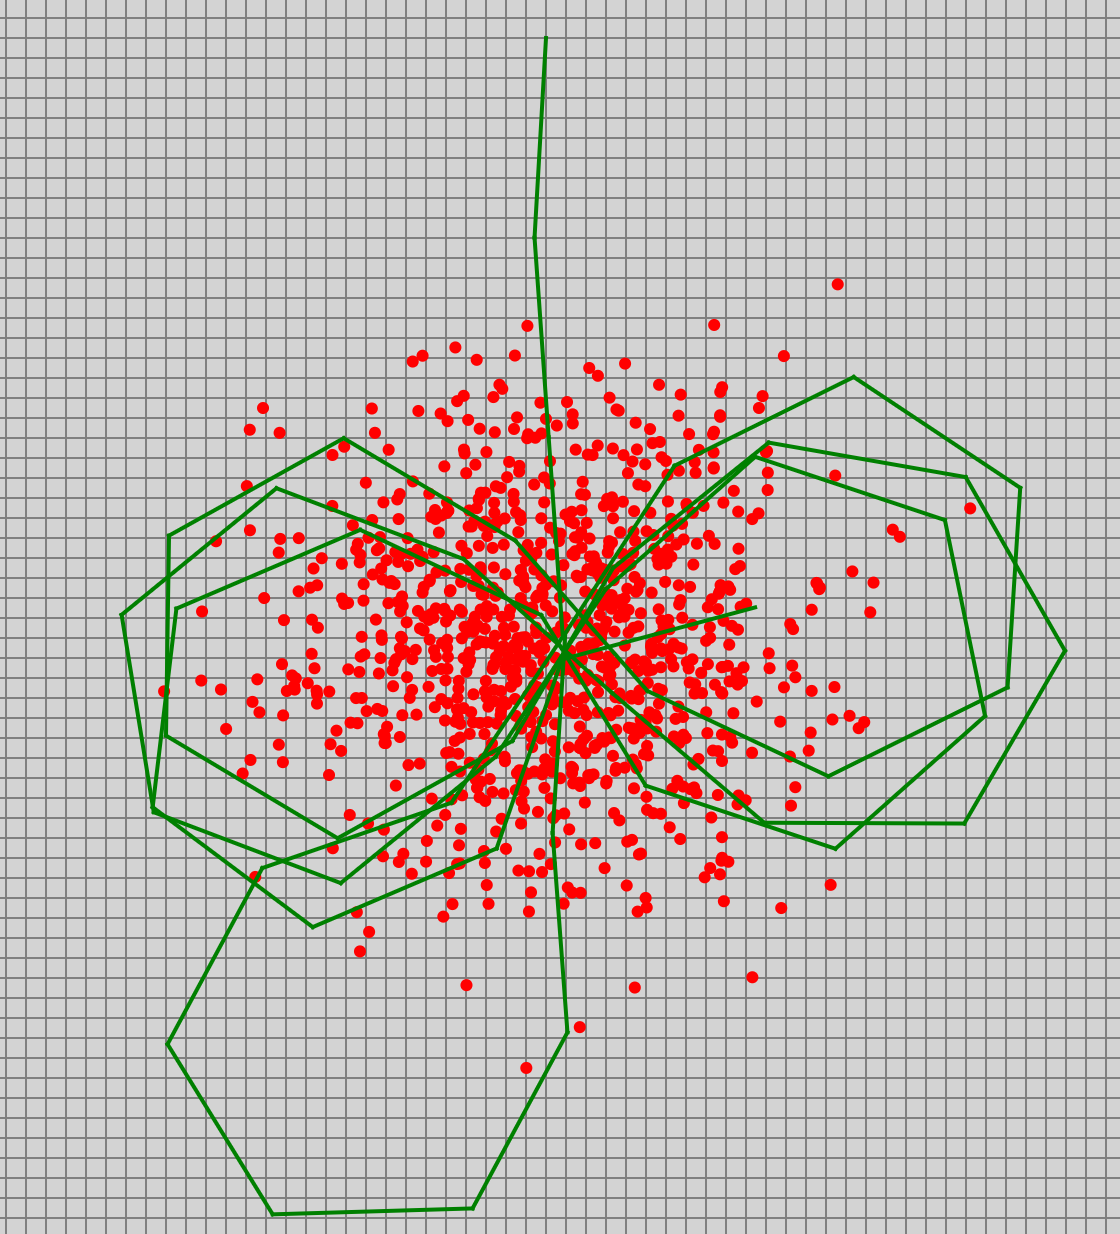
\includegraphics[width=0.6\linewidth]{goodRouteScenario1.png}
	\centering
	\label{fig:scenario1Good}	
	\end{figure}

Figures~\ref{fig:scenario1Poor} and~\ref{fig:scenario1Good} show an example of a poor and good route generated by the proposed algorithm for this scenario. 
The path of the poor route travels far from the distribution of particles, which suggests that the algorithm gets stuck converging too early and lacks diversity in the population to move towards a more central route plan.

This adds weight to the fast convergence hypothesis proposed as an explanation for the reason why decoding the waypoints is not beneficial.
The search space is effectively twice as large in decoded space. The algorithms with decoded waypoints might be quickly converging on the waypoints in the initial population, but in doing so cutting down on the number of generations of exploration and soon loose diversity.

The good example of a route from the first scenario (also generated by the proposed algorithm) flies in a figure of 8 over the centre point of the distribution.
This is an excellent search strategy for such a scenario, which is very similar to a standard search pattern called sector search, often carried out at the beginning of a search and rescue operation over the last known point of communication.

Examples of good and poor routes from scenarios 2 and 3 can also be seen in figures~\ref{fig:scenario2Good}-\ref{fig:scenario3Poor}. In the poor example from scenario 2, the route fails to explore the north west distribution, which contributes significantly to its worse fitness.
Again, this suggests that the algorithm is converging too quickly without fully exploring the search space.

In scenario 3, the poor example is greedy again, staying mostly in-between the two closest distributions. It can further be observed that even routes with the best fitness in this scenario fail to explore the north eastern distribution.
		
	%JADE
\begin{figure}[t]
	\caption{Scenario 2 - Example of Good Route ($\overline{P}_s(t_m)=0.6739$)}
	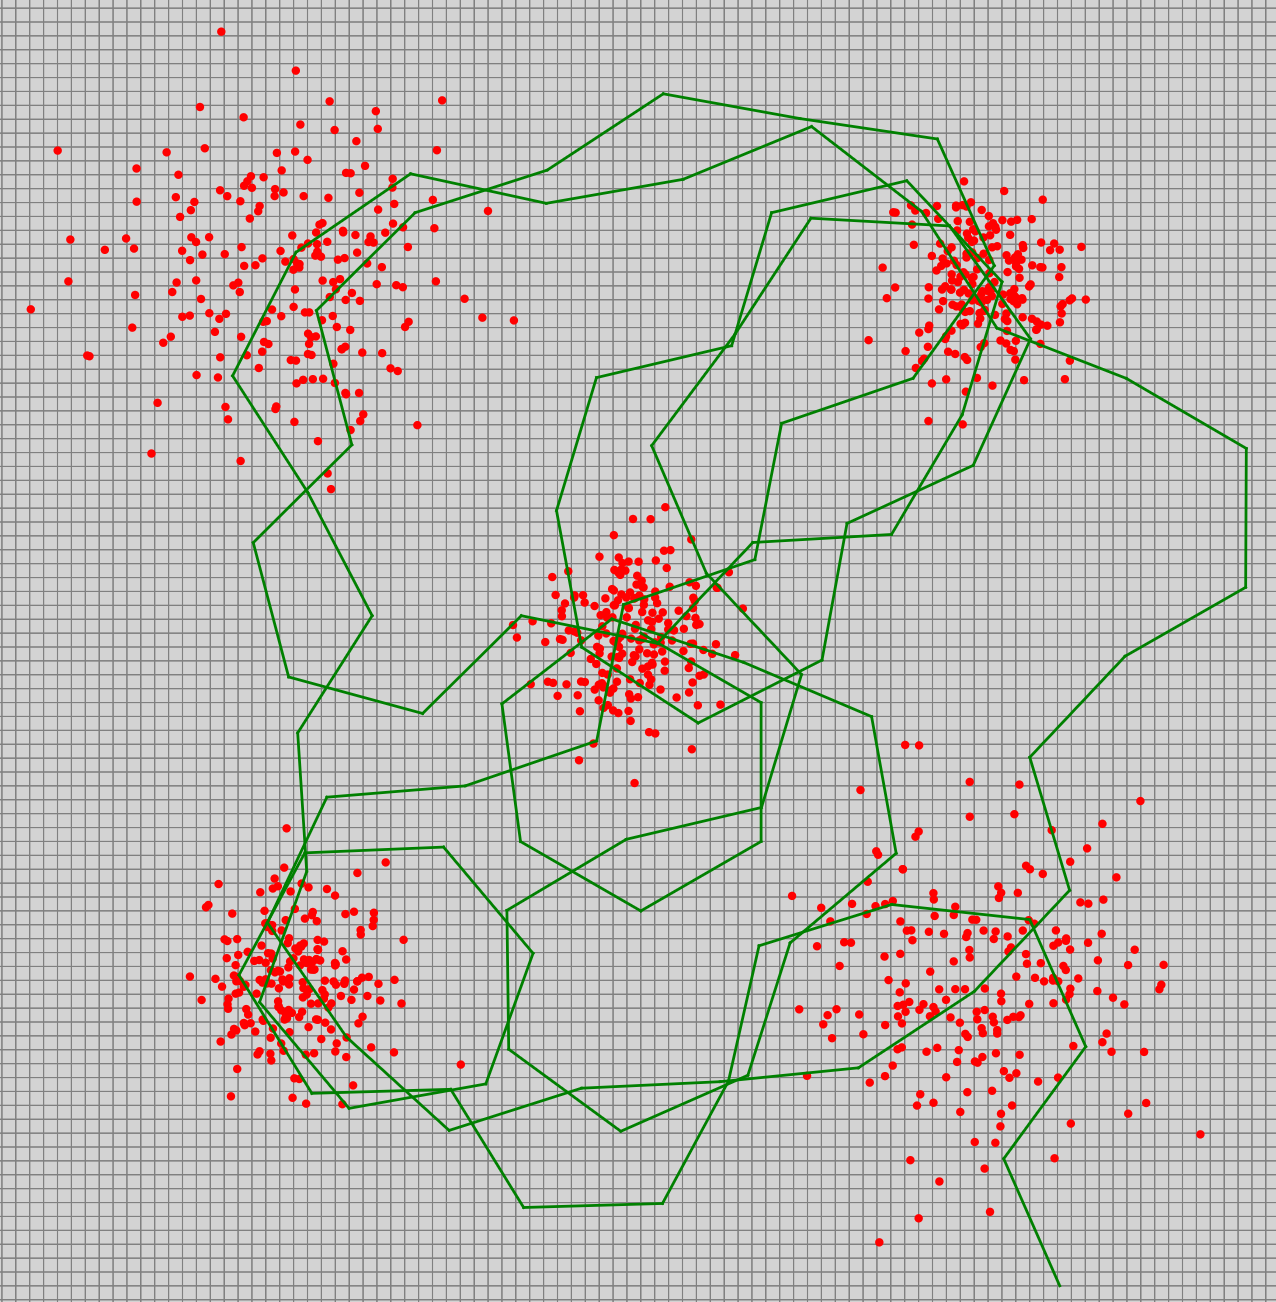
\includegraphics[width=0.7\linewidth]{goodRouteScenario2.png}
	\centering
	\label{fig:scenario2Good}	
	\end{figure}	
	
	%proposed
	\begin{figure}[t]
	\caption{Scenario 2 - Example of Poor Route ($\overline{P}_s(t_m)=0.7263$)}
	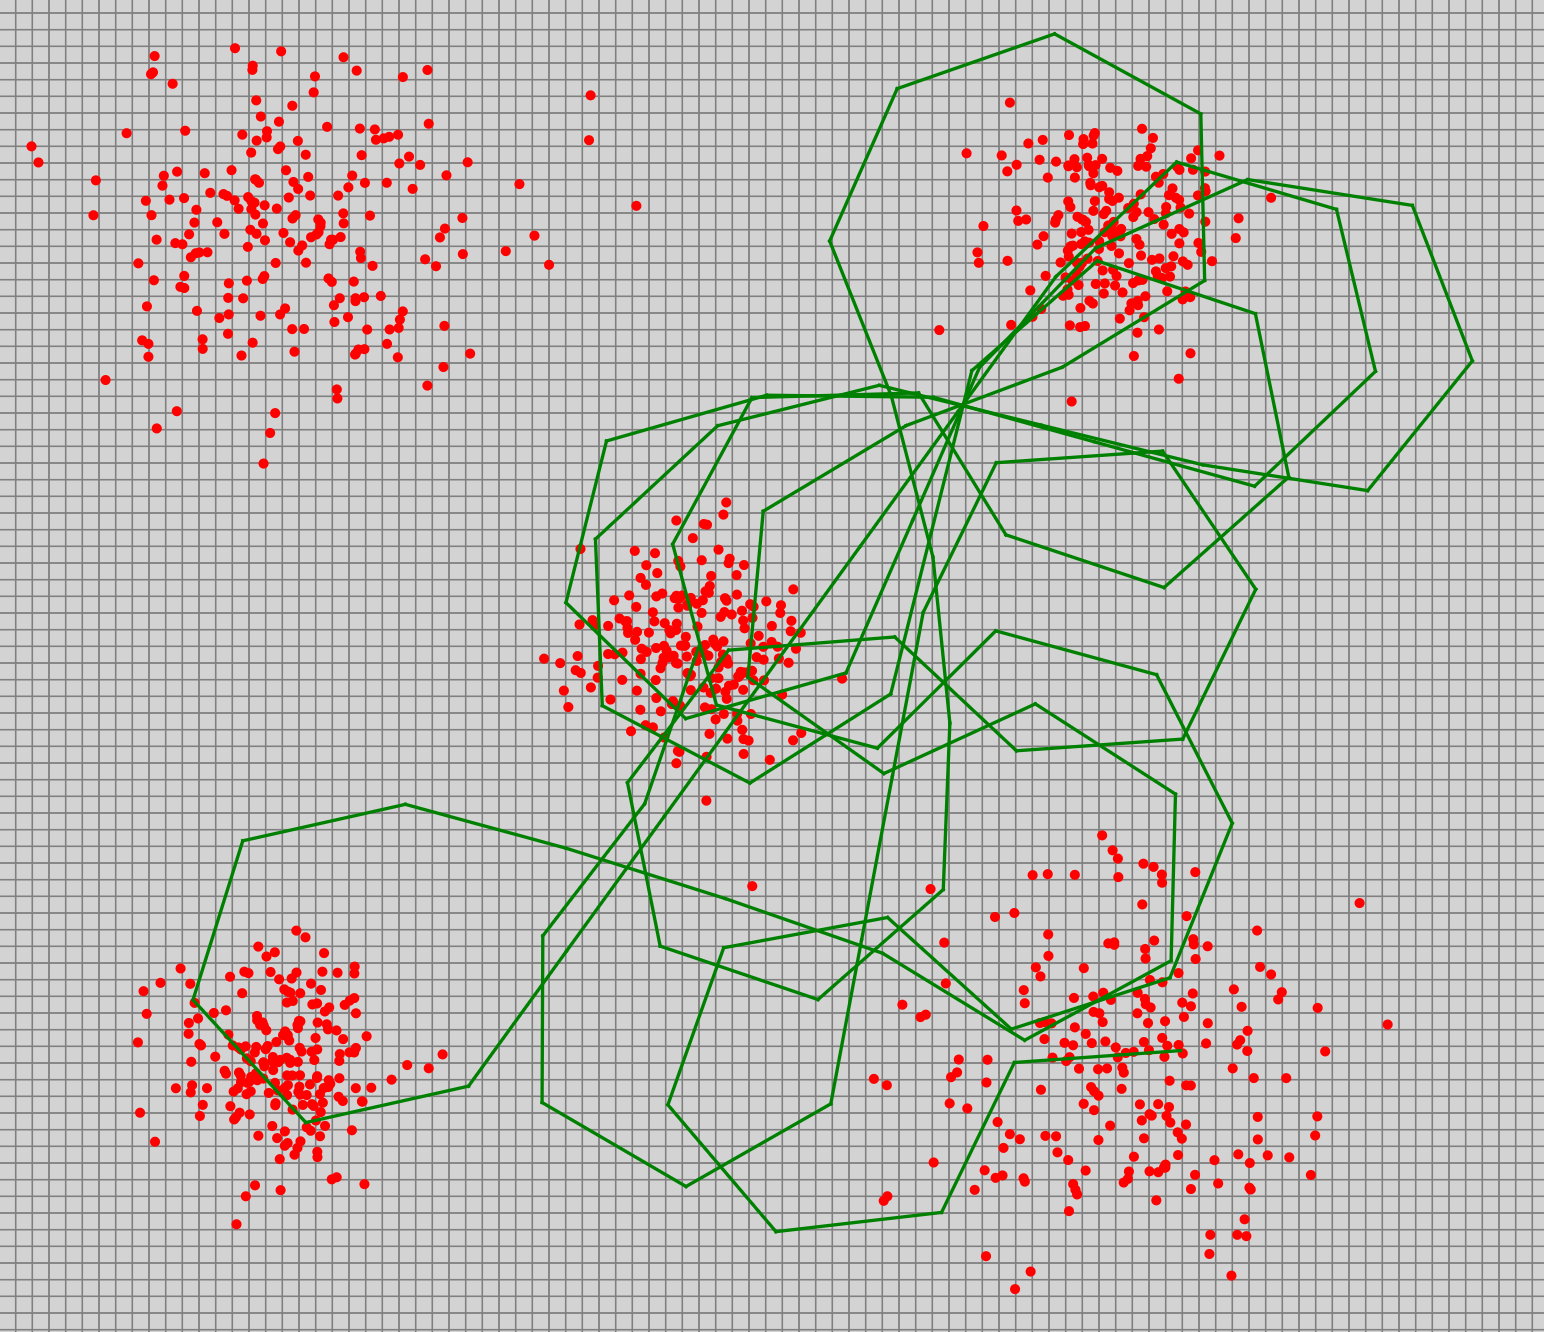
\includegraphics[width=0.7\linewidth]{poorRouteScenario2.png}
	\centering
	\label{fig:scenario2Poor}	
	\end{figure}	
	
	%JADE
\begin{figure}[t]
	\caption{Scenario 3 - Example of Good Route ($\overline{P}_s(t_m)=0.7402$)}
	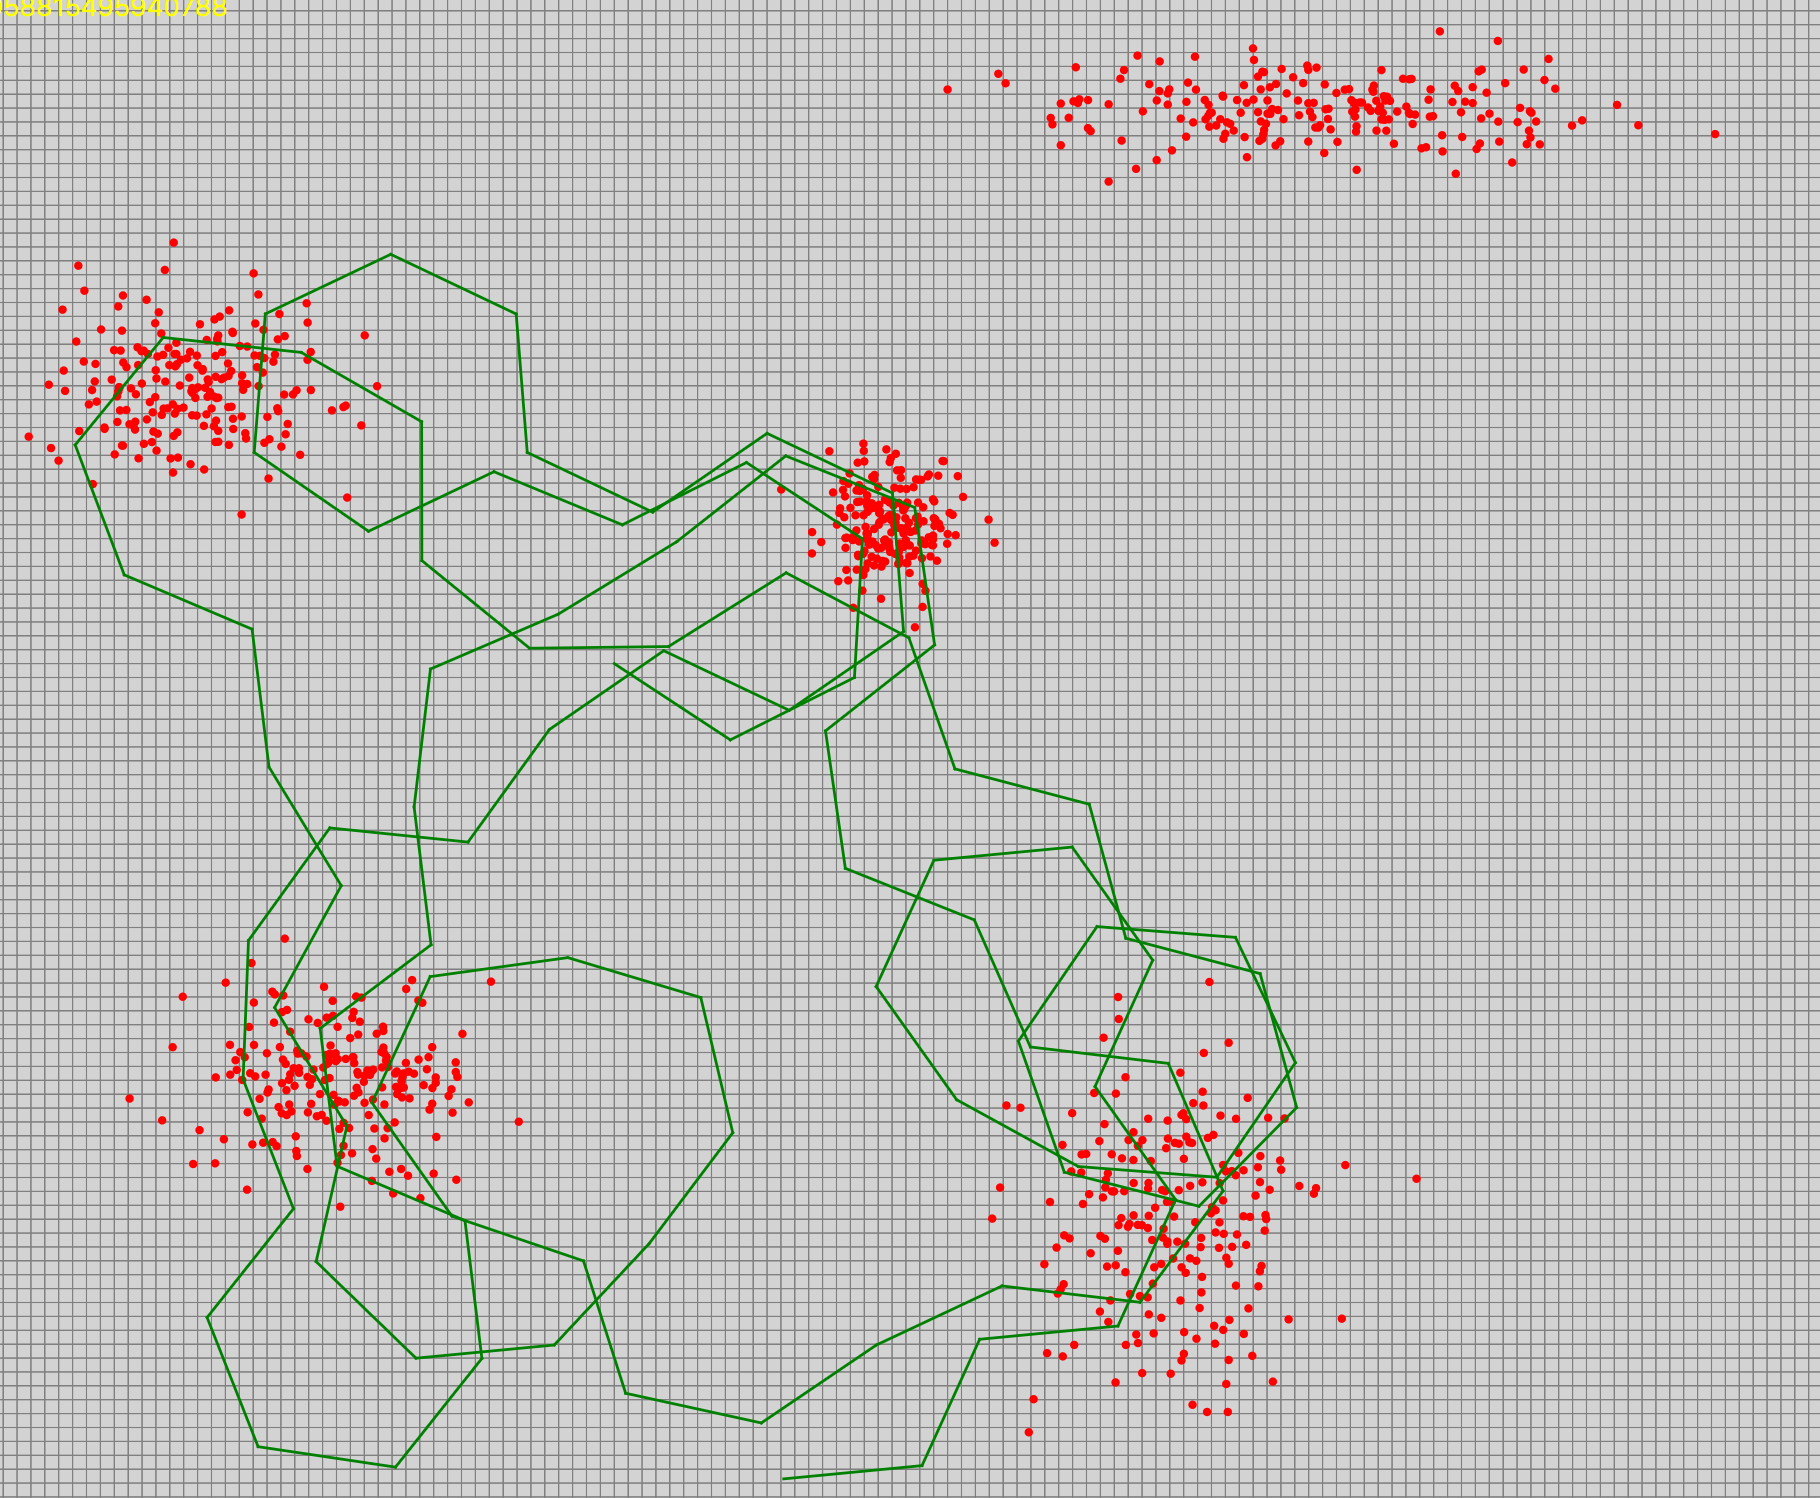
\includegraphics[width=0.7\linewidth]{goodRouteScenario3.png}
	\centering
	\label{fig:scenario3Good}	
	\end{figure}	
	
	%proposed
	\begin{figure}[t]
	\caption{Scenario 3 - Example of Poor Route ($\overline{P}_s(t_m)=0.8081$)}
	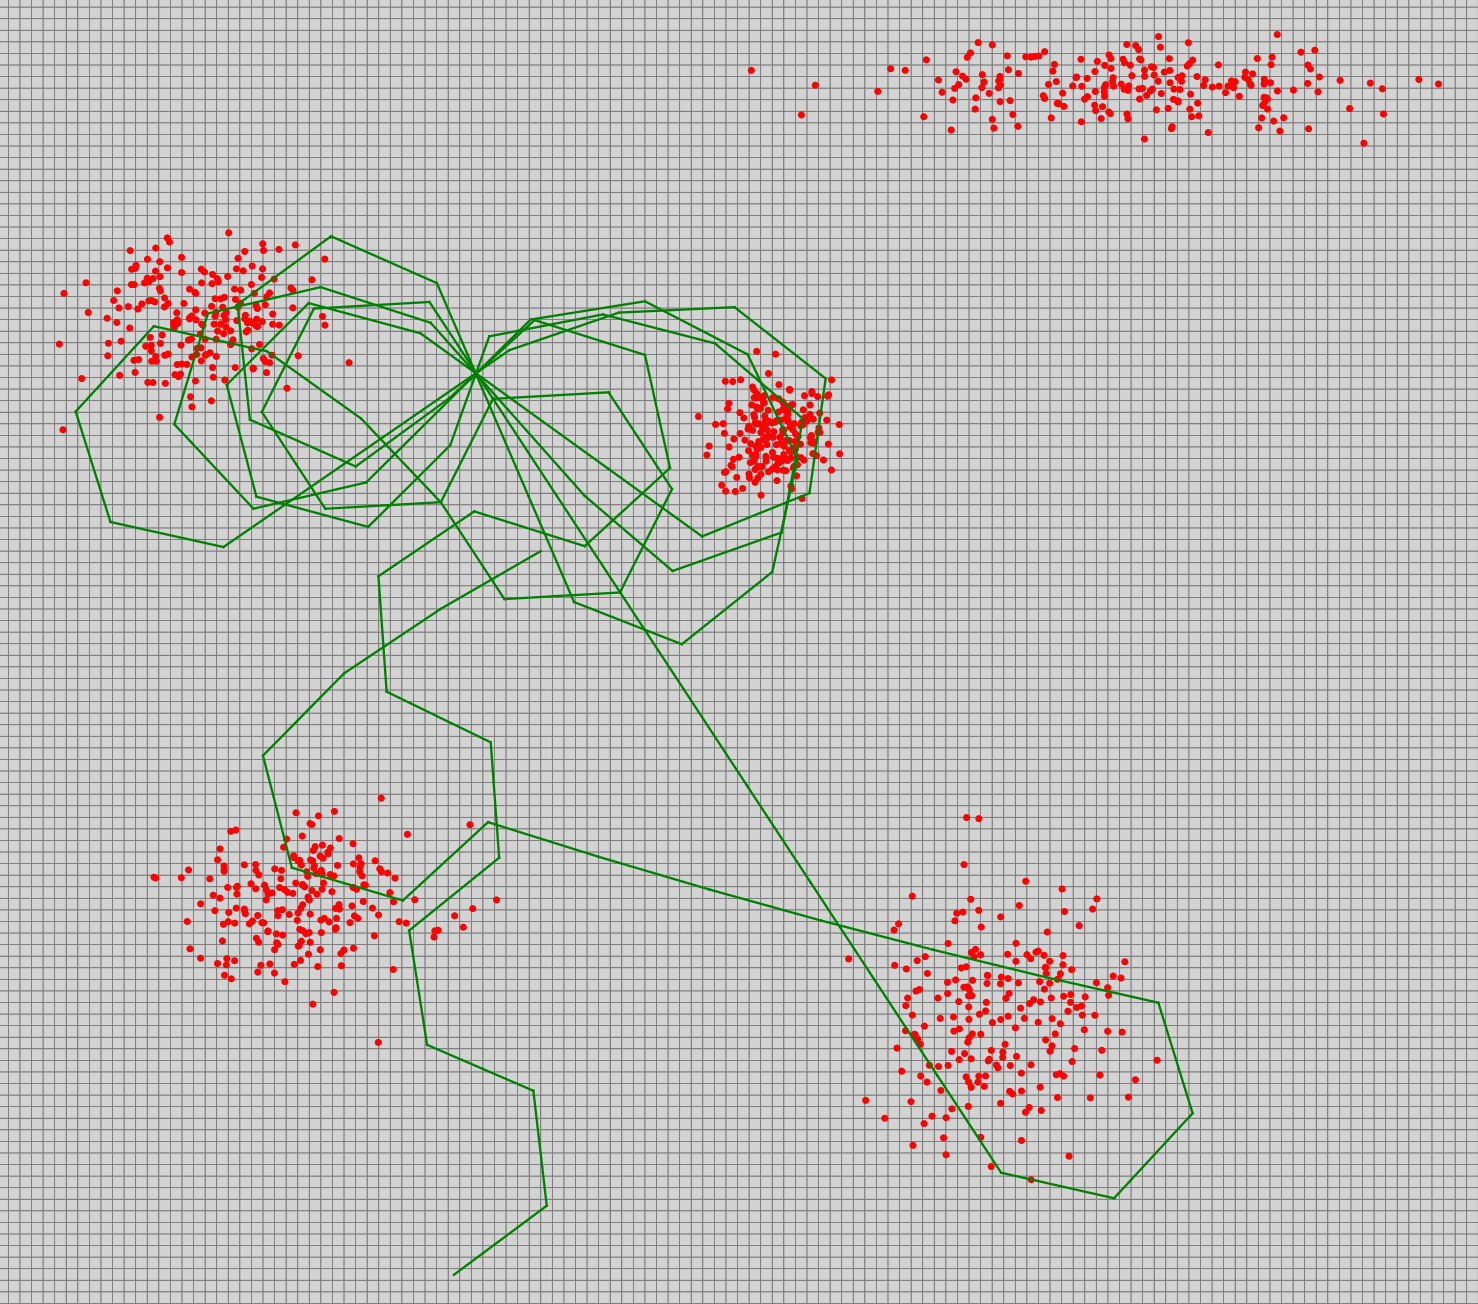
\includegraphics[width=0.7\linewidth]{poorRouteScenario3.png}
	\centering
	\label{fig:scenario3Poor}	
	\end{figure}	
	
\begin{figure}[H]
	\caption{Median Fitness Convergence - Scenario 1}
	\centering
	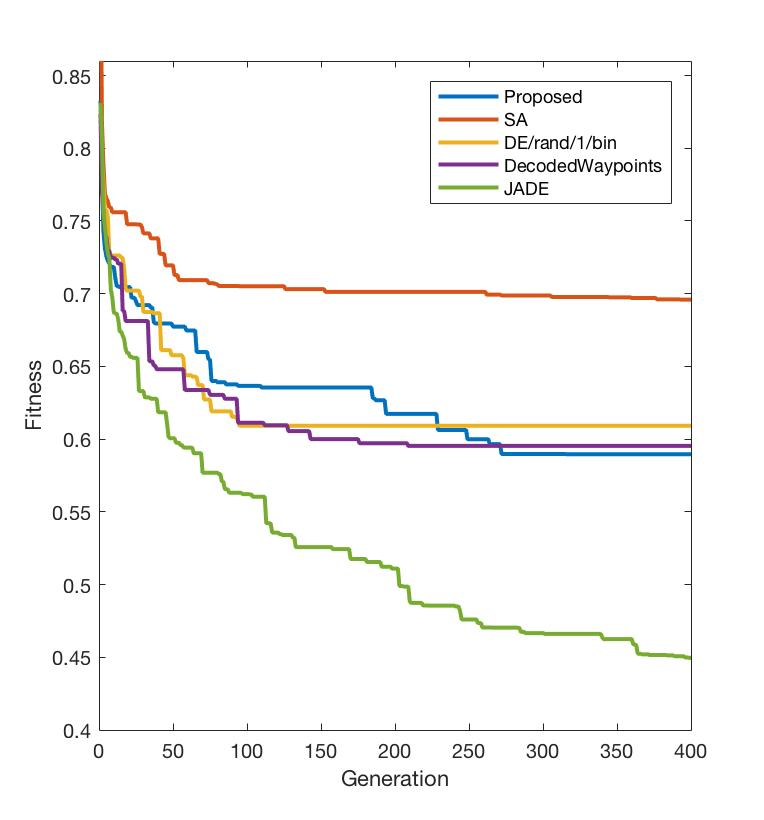
\includegraphics[width=0.7\linewidth]{scenario1Plot.jpg}
	\label{fig:medianPlot1}	
	\end{figure}
	
		\begin{figure}[H]
	\caption{Median Fitness Convergence - Scenario 2}
	\centering
	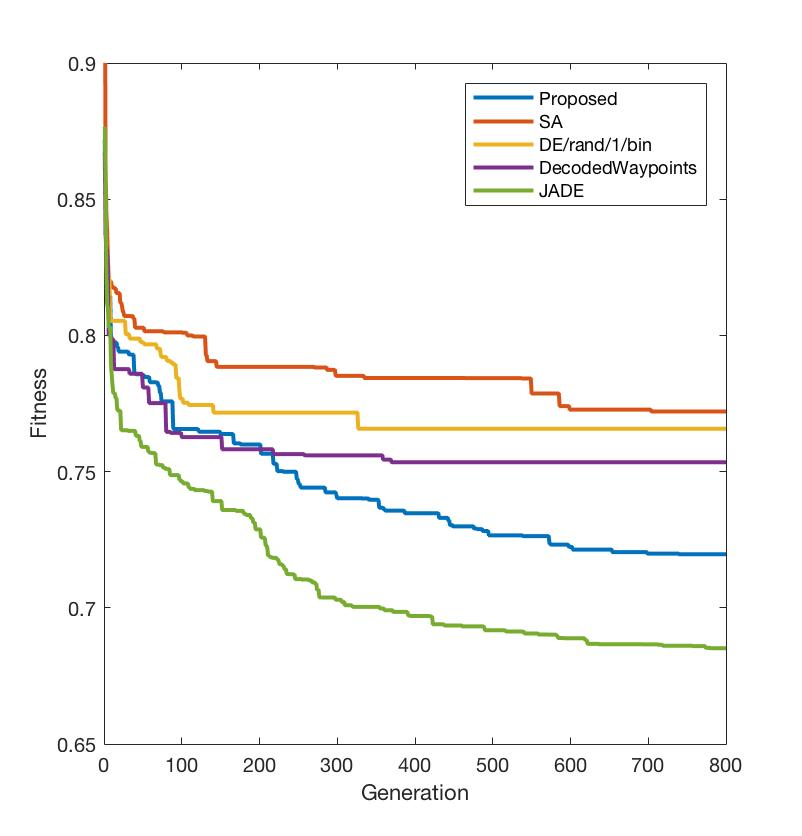
\includegraphics[width=0.7\linewidth]{scenario2Plot.jpg}
	\label{fig:medianPlot2}	
	\end{figure}
	
\begin{figure}[t]
	\caption{Median Fitness Convergence - Scenario 3}
	\centering
	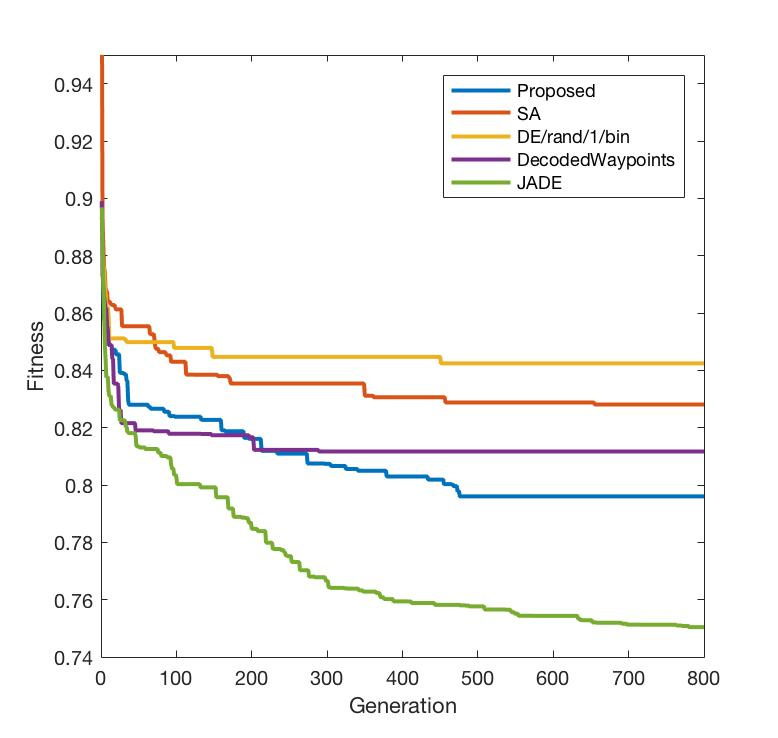
\includegraphics[width=0.7\linewidth]{scenario3Plot.jpg}
	\label{fig:medianPlot3}	
	\end{figure}	
	
The graphs in figures~\ref{fig:medianPlot1},~\ref{fig:medianPlot2} and~\ref{fig:medianPlot3} show the median fitness from all runs after each generation for the three scenarios respectively.
Again, JADE is clearly most effective with a very quick convergence during the initial generations and then slowing to a steady rate of improvement towards the final generations.
The convergence of the proposed algorithm appears to slow significantly early on, with scenario 3 showing no further improvements after 500 generations.
Again this could imply that JADE without decoded waypoints has more effective early exploration.

The route freezing alteration seems most beneficial in the more complex scenarios, especially in the later generations.
This suggests the contrary, that the decoded waypoints algorithm stagnates as it attempts to mutate too many early waypoints affecting the fitness of later ones.
By focussing later generations of search on temporally more distant waypoints, essentially fixing the earlier route in place, allows the algorithm to exploit the latter part of the route more effectively.
	
	\section{Conclusions and Discussion}	
	\label{section:conclusion}
	
	The results seem to imply that the approach taken to defining the problem of route planning for UAV search and rescue missions as a continuous single-objective optimisation is able to produce a number of quality solutions with the simple scenarios defined.
	While the algorithmic work requires some more analysis, the approach lends itself to be easily extended to more complex scenarios.
	
	The proposed alteration to JADE of freezing the routes in later generations appears to be beneficial to the algorithm in all three of the simulation scenarios.
	It is disappointing, however, that the proposed alteration of decoding the routes into waypoints before mutation appears to be detrimental.
	
	Both of the proposed alterations to JADE are aimed at tackling stagnation.
	Decoding the waypoints allows the algorithm to converge more effectively, while temporal route freezing prevents stagnation by restricting the search space in later generations.
	It is curious then, that one alteration seems to hinder performance, while the other improves it.
	It could be that early generations of the search are essential for exploration, and so by speeding up convergence here, culls the diversity required to explore effectively. Later generations of the search are then prone to stagnation as the fitness of more distant waypoints is so greatly affected by altering the earlier waypoints.
	
	More analysis is required to confirm this hypothesis, which could be achieved by inspecting the candidate routes at each generation using the visualisation tool.
	It would also be useful to implement a version of JADE with route freezing and no decoded waypoints to understand whether this alteration alone is beneficial to the optimisation.
	
	In suggested in~\cite{Yang2016} that using a MMOA approach might also be beneficial in exploring multiple modes simultaneously without stagnating due to cross-over between them.
	Other algorithmic approaches such as ACO have also demonstrated some promising results in the field of path planning for UAVs, so future work could also include implementing a version of such an algorithm for the context of search and rescue planning.
	
	 Finally, the scenarios chosen in this paper are relatively simplistic as the distributions remain constant throughout the path plan.
	 In real world planning, it is potentially the changing distribution of probability that adds such significant difficulty to the mission planning problem.
	 As mentioned, further work could be carried out to extend this approach to such scenarios by incorporating an ocean drift model to further prove the effectiveness of the approach to realistic S\&R planning scenarios.
	
%	\subsection{Future Work}
%		
%		More types of problem
%		Would be good to visualise each generation.
%		Compare against ant colonisation..?
%		Isolate route freezing.
%		Moving distribution
%		
%		Heirarchical search (start with less waypoints and then refine)		 Goodrich paper!
%		
%		Direct comparison with discrete approaches?
%	Time analysis
%	apply ideas from lin2009	
%	

	
	\bibliographystyle{ieeetr}
	\bibliography{myReferences} 	
	
	\clearpage
	\onecolumn
	\begin{appendices}
	\section{Integrating the Inverse Cubed Law of Visual Detection Between Two Waypoints}
	\label{appendix:integratingInverseCubedLaw}
	
With stationary particle $\rho_i$ at location $(x_{i},y_{i})$,  waypoint $w_j$ at time $t=t_j$ and location $(x_{j},y_{j})$ to waypoint $w_{j+1}$ at time $t=t_{j+1}$ and location $(x_{j+1},y_{j+1})$, and constant altitude $h$, the instantaneous horizontal distance $r$ from the particle to the UAV at time $t$ (where $t_j\leq t \leq t_{j+1}$) is calculated:

\begin{equation}
	\label{equation:particleWpDistanceAppendix}
\begin{split}
r = (((x_{w^j}-x_{p^i})+(x_{w^{j+1}}-x_{w^j}) t)^2\\
 + ((y_{w^j}-y_{p^i})+(y_{w^{j+1}}-y_{w^j}) t)^2)^{1/2}
\end{split}
\end{equation}	
	
Let us denote:

$$
a=x_{w^j}-x_{p^i}
$$	

$$
b=x_{w^{j+1}}-x_{w^j}
$$

$$
c=y_{w^j}-y_{p^i}
$$

$$
d=y_{w^{j+1}}-y_{w^j}
$$

The instantaneous probability of detection $\gamma$ from (\ref{equation:horizontalInverseSquareLaw}), becomes:

	\begin{equation}
	\label{equation:horizontalInverseSquareLawBetweenWPs}
	\gamma = \frac{kh}{((a+bt)^2+(c+dt)^2+h^2)^{3/2}}
	\end{equation}
	
	So, finally: 
	\begin{equation}
	\int_{t_j}^{t_{j+1}} \gamma(t)dt=\int_{t_j}^{t_{j+1}}\frac{kh}{((a+bt)^2+(c+dt)^2+h^2)^{3/2}}dt
	\end{equation}
	\begin{equation}
	\int_{t_j}^{t_{j+1}} \gamma(t)dt=\left[-\frac{kh(ab+cd+2t)}{(a^2(b^2-2)+2abcd+c^2(d^2-2)-2h^2)\sqrt{a^2+2abt+c^2+2cdt+h^2+2t^2}}\right]_{t_j}^{t_{j+1}}
	\end{equation}
	
	\end{appendices}
	
\end{document}